% !TeX spellcheck = en_US
% Dirty hack to disable recompiling the bibliography every time, reducing compilation times. Comment out to re-compile bibliography.
% !TeX TXS-program:recompile-bibliography = donothing

% Use biber as bibliography tool
% !TeX TXS-program:bibliography = txs:///biber

\documentclass[a4paper]{scrreprt}

\usepackage{xargs}                      % Use more than one optional parameter in a new commands
\usepackage[pdftex,dvipsnames]{xcolor}  % Coloured text etc.
\usepackage[colorinlistoftodos,prependcaption,textsize=tiny]{todonotes}
\newcommandx{\error}[2][1=]{\todo[linecolor=red,backgroundcolor=red!25,bordercolor=red,#1]{#2}}
\newcommandx{\unsure}[2][1=]{\todo[linecolor=orange,backgroundcolor=orange!25,bordercolor=orange,#1]{#2}}
\newcommandx{\change}[2][1=]{\todo[linecolor=blue,backgroundcolor=blue!25,bordercolor=blue,#1]{#2}}
\newcommandx{\info}[2][1=]{\todo[linecolor=OliveGreen,backgroundcolor=OliveGreen!25,bordercolor=OliveGreen,#1]{#2}}
\newcommandx{\improvement}[2][1=]{\todo[linecolor=Plum,backgroundcolor=Plum!25,bordercolor=Plum,#1]{#2}}
\newcommandx{\thiswillnotshow}[2][1=]{\todo[disable,#1]{#2}}


\usepackage{amsfonts} 
\usepackage{amsmath}
\usepackage{amsthm} %Proof Environment
\usepackage{amssymb}
\usepackage{marvosym}
\usepackage{stmaryrd} %\lightning
\usepackage{latexsym} %\leadsto

\usepackage[utf8]{inputenc}
\usepackage[T1]{fontenc}
\usepackage[english]{babel} 

\usepackage{pdfpages} % include pdf pages
\usepackage{hyperref}
\usepackage{graphicx}

\usepackage{enumitem}
\usepackage{multicol}
\usepackage{chngcntr}

\usepackage{xifthen}

\usepackage{listings} % source listings
\usepackage{xcolor} % defining own colors: \color

\usepackage{dsfont} % \1 for identity functions

\usepackage{etoolbox}

% custom math commands:

% column vectors
\newcount\xveccount
\renewcommand*\vec[1]{
	\global\xveccount#1
	\begin{pmatrix}
		\vecnext
	}
	\def\vecnext#1{
		#1
		\global\advance\xveccount-1
		\ifnum\xveccount>0
		\\
		\expandafter\vecnext
		\else
	\end{pmatrix}
	\fi
}  
\newcommand{\vectwo}[3][0pt]{\begin{pmatrix}#2\\[#1] #3\end{pmatrix}}
\newcommand{\vecthree}[4][0pt]{\begin{pmatrix}#2\\[#1] #3\\[#1] #4\end{pmatrix}}
\newcommand{\vecfour}[5][0pt]{\begin{pmatrix}#2\\[#1] #3\\[#1] #4\\[#1] #5\end{pmatrix}}
\newcommand{\vecfive}[6][0pt]{\begin{pmatrix}#2\\[#1] #3\\[#1] #4\\[#1] #5\\[#1] #6\end{pmatrix}}

% * as multiplication dot
\mathcode`\*="8000
{\catcode`\*\active\gdef*{\cdot}}

% common number set symbols
\newcommand{\N}{\mathbb{N}}
\newcommand{\Z}{\mathbb{Z}}
\newcommand{\Q}{\mathbb{Q}}
\newcommand{\R}{\mathbb{R}}
\newcommand{\C}{\mathbb{C}}

% useful mathematical operators
\DeclareMathOperator{\Pot}{\mathcal{P}}
\DeclareMathOperator{\BigO}{\mathcal{O}}
\DeclareMathOperator{\inv}{^{-1}}
\renewcommand{\Re}[1]{\text{Re}\left( #1 \right)}
\renewcommand{\Im}[1]{\text{Im}\left( #1 \right)}
\newcommand{\abs}[1]{\left| #1 \right|}
\DeclareMathOperator{\vspan}{\text{span}}
\newcommand{\setspan}[1]{\vspan\left(\left\{#1\right\}\right)}
\DeclareMathOperator{\rang}{\text{rang}}
\newcommand{\integral}[4]{\int_{#1}^{#2} #3 \, d#4}
\newcommand{\lintegral}[3]{\int_{#1} #2 \, d#3}
\newcommand{\comp}{^\complement}
\newcommand{\ra}{\rightarrow}
\newcommand{\lra}{\Leftrightarrow} % equivalence arrow
\newcommand{\1}[1][]{\mathds{1}\ifthenelse{\isempty{#1}}{}{_{#1}}}
\newcommand{\dummydot}{\,\cdot\,}
\DeclareMathOperator{\im}{\text{im}}
\newcommand{\innerprod}[2]{\left\langle #1, #2 \right\rangle}
\DeclareMathOperator{\supp}{supp}
\newcommand{\transposed}{^{T}}
\DeclareMathOperator{\argmax}{argmax}
\DeclareMathOperator{\argmin}{argmin}
\newcommand{\colonlra}{\mathrel{\vcentcolon\Leftrightarrow}} % properly typeset :<=>

% switch-case structure
\newcommand{\ifequals}[4]{\ifthenelse{\equal{#1}{#2}}{#3}{#4}}
\newcommand{\case}{} % Dummy, so \renewcommand has something to overwrite...
\newenvironment{switch}[1]{\renewcommand{\case}[3]{\ifequals{#1}{##1}{##2}{##3}}}{} %Usage: \begin{switch}{value}, \case{value}{then}{else}

% shortcut for inline pmatrix
\newcommand{\pmat}[1]{\begin{pmatrix}#1\end{pmatrix}}

% brutally enforce centering the contents
\newcommand{\centerbrutally}[1]
{
	\centerline{
		\begin{minipage}{\linewidth}
			#1
	\end{minipage}}
}

\definecolor{verylightgray}{gray}{0.97}
\definecolor{purple}{RGB}{127,0,116} % used for keyword coloring in source code listings
\definecolor{brickred}{rgb}{0.56, 0.175, 0.231} % used for string coloring in source code listing

% norm ||x||
\newcommand{\norm}[1]{\left\lVert#1\right\rVert}

% centered inline graphics
\newcommand{\includegraphicsinline}[2][]{\begingroup\setbox0=\hbox{\includegraphics[#1]{#2}}\parbox{\wd0}{\box0}\endgroup}

% tilde in lstlisting
\lstset{literate=%
    {~}{{\textasciitilde}}1
}

% shortcuts: for limits/series going to infinity
\newcommand{\liminfty}[1]{\lim\limits_{#1 \rightarrow \infty}}
\newcommand{\ser}[1]{\sum\limits_{\ifthenelse{\isin{=}{#1}}{#1}{#1=1}}^{\infty}}
\newcommand{\toinfty}[1]{\xrightarrow{\;#1 \to \infty\;}}

% shortcut for multiple cases in math formulas: '"1", falls "2", "3", falls "4"' (bzw. 'sonst', falls leer)
\newcommand{\twocases}[4]
{
    \begin{cases}
        #1, &\text{if } #2 \\
        #3, &\ifthenelse{\isempty{#4}}{\text{else}}{\text{if } #4}
    \end{cases}
}

% shortcut for parentheses and sets
\newcommand{\pars}[1]{\left(#1\right)}
\newcommand{\bigpars}[1]{\bigl(#1\bigr)}
\newcommand{\biggpars}[1]{\biggl(#1\biggr)}
\newcommand{\set}[1]{\{#1\}}
\newcommand{\bigset}[1]{\bigl\{#1\bigr\}}
\newcommand{\biggset}[1]{\biggl\{#1\biggr\}}
\newcommand{\bigmid}{\bigm\vert}
\newcommand{\biggmid}{\biggm\vert}

\newenvironment{correction}[1]{\color{red}\textbf{\underline{#1}}\\}{\ignorespacesafterend}

\makeatletter
\patchcmd{\upbracefill}{\m@th}{\scriptscriptstyle\m@th}{}{}
\patchcmd{\upbracefill}{$\braceld$}{$\scriptstyle\braceld$}{}{}
\patchcmd{\upbracefill}{\bracelu}{\bracelu\mkern-1mu}{}{}
\patchcmd{\upbracefill}{\hfill\braceru}{\hfill\mkern-1mu\braceru}{}{}
\makeatother

\newcommand{\smallmat}[1]{\left(\begin{smallmatrix}#1\end{smallmatrix}\right)}
\newcommand{\undersetbrace}[2]{\underset{#2}{\underbrace{#1}}}

% theorem-like environments

\theoremstyle{definition}
\newtheorem{thm}{Theorem}[chapter] % reset theorem numbering for each chapter
\newtheorem*{thm*}{Theorem}
\newtheorem{defn}[thm]{Definition} % definition numbers are dependent on theorem numbers
\newtheorem*{defn*}{Definition}
\newtheorem{ex}[thm]{Example} % same for example numbers
\newtheorem*{ex*}{Example}
\newtheorem{lemma}[thm]{Lemma} % same for Lemma numbers
\newtheorem*{lemma*}{Lemma}
\newtheorem{cor}[thm]{Corollary}
\newtheorem*{cor*}{Corollary}
\newtheorem{comm}[thm]{Comment}
\newtheorem*{comm*}{Comment}
\newtheorem{notation}[thm]{Notation}
\newtheorem*{notation*}{Notation}


\usepackage[citestyle=alphabetic,bibstyle=alphabetic]{biblatex}
\usepackage{csquotes} % needed for biblatex

\usepackage{setspace}
\usepackage[headsepline]{scrlayer-scrpage}
\usepackage{mathtools} % \bigtimes

% no ident, combined with reasonable paragraph spacing
\onehalfspacing
\setlength{\parindent}{0em}
\setlength{\parskip}{1.7ex}

\addbibresource{Bachelor-Thesis.bib}

\DeclareMathOperator{\A}{\mathcal{A}}
\DeclareMathOperator{\F}{\mathcal{F}}
\newcommand{\Rp}{\mathbb{R}_+}
\let\epsilon\varepsilon
\let\phi\varphi
\newcommand{\B}{\mathcal{B}}
\newcommand{\D}{\mathcal{D}}

\ihead{Vincent Bürgin}
\ohead{[Work in Progress]}

\begin{document}
    \tableofcontents
    
    \chapter{Introduction}
    
    % TODO make the following one chapter?
    \chapter{Basic Concepts from Probability and Decision Theory}
    
    \section{Probability Theory}
    
    \section{Decision Theory}
    
    
    \chapter{Non-Cooperative Game Theory}
    \label{chap:nonCooperativeRealValuedGameTheory}
    In this chapter, we will have a look at the basic notions of non-cooperative game theory.
    Game theory is applied in scenarios where multiple agents, called \emph{players}, make decisions independently of another, and each try to achieve the best outcome for themselves.
    We are explicitly excluding \emph{cooperative game theory} from our discussions, where the players can cooperate and form coalitions to achieve a better overall outcome, and the main issue is how to split up the common payoff between the players.
    In the \emph{non-cooperative game theory} we are dealing with, on the other hand, players can be thought of as neither being able to communicate, nor to make binding agreements. 
    The classical example of this is the prisoners dilemma:
    \begin{ex}[Prisoner's Dilemma]
        Two criminals have committed a capital crime together. They were caught, and now are being held in different cells, with no way to communicate, and will soon be interrogated.
        They know, however, that law enforcement only has substantial evidence against them for a small part of the crime; if none of the two confess, both of them will only be sentenced to one year in prison.
        The dilemma is that both will be offered to confess to the crime, and also snitch on the other criminal. Now if one of them confesses and testifies against the other, he can be placed in a witness protection program and go free, while the other one will go to prison for five years. If both confess, however, they will both be sentenced to four years in prison, with their confession being held for them as mitigating circumstances.
        
        The game can be represented by a matrix, where the years in prison for the first and second player, respectively, are given as vectors:
        The rows are the possible actions of player 1, the columns the actions of player 2 (not confess vs. confess).
        
        \begin{table*}[h]
            \centering
            $\begin{pmatrix}
                (1, 1) & (5, 0) \\
                (0, 5) & (4, 4)
            \end{pmatrix}$
        \end{table*}
    
        Obviously if the prisoners could make a binding agreement, they would be best of by both not confessing, and both only facing one year in prison.
        However, if one prisoner does not confess, he risks being ratted out by the other prisoner and face even more time in prison; 
        Therefore, somewhat counter-intuitively, the non-cooperative game theorist's solution is that both prisoners confess and both face four years in prison instead of just one, only to prevent being betrayed by the other prisoner.
        \label{ex:prisonersDilemma}
        \label{ex:gameTheoryIntroductoryExample}
    \end{ex}

    We will now define such games formally.

    % TODO find a definition properly supported by the literature!
    % TODO really one-shot? Not better strategic-form? Multi-Stage games can also be encoded like this...
    % TODO from now on, we call these games
    \begin{defn}
        A \emph{real-valued one-shot simultaneous move game} $(n, (S_1, \dots, S_n), (u_1, \dots, u_n))$ consists of 
        \begin{itemize}
            \item the number of players $n$,
            \item for each player $k$, a set $S_k$ of available strategies,
            \item for each player $k$, a payoff function $u_k: S \to \R$, where $S = \bigtimes\limits_{1\leq i \leq n} S_i$ denotes the set of all possible combinations of the players' strategies (elements of $S$ are also called \emph{strategy profiles}). 
        \end{itemize}
        \label{defn:realValuedGames}
    \end{defn}
    
    Instead of specifying payoff functions $u_k$, we could equivalently specify cost functions $c_k$ with the semantics that players want to maximize payoffs, but minimize costs. We can switch between those viewpoints by setting $u_k = - c_k$. For a strategy profile $s = (s_1, \dots, s_n) \in S$ and some player $k$, it is sometimes convenient to use the notation $s_{-k}$ for $s$ with the $k$'th coordinate left out, and write $u_k(s_k, s_{-k})$ instead of $u_k(s)$.
    % TODO “and we will use what is most convenient; but mean payoffs unless noted otherwise”?
    
    A common special case are zero-sum games:
    
    \begin{defn}
        A \emph{two-player zero-sum game} is a game which has two players, and 
        \[ \forall s \in S: u_1(s) + u_2(s) = 0 \]
    \end{defn}

    In a zero-sum game, the two players are completely antagonistic: % TODO formally justify this term?
    one player wins exactly what the other loses, and there would be no reason for the players to cooperate in any way. As \cite{bib:fudenbergGameTheory} notes, the important feature of these games is that the payoffs sum to a constant, while choosing this constant as zero is only for normalization.
    
    \section{Solution Concepts}
    Reasoning about rational strategies, as done in example \ref{ex:gameTheoryIntroductoryExample}, is formalized by \emph{solution concepts}, most prominently the concept of \emph{Nash equilibria}. The first, somewhat simpler concept is that of \emph{dominant strategies}, where the best strategy is optimal regardless of the other players' actions:
    
    \begin{defn}[Dominant strategy]
        A strategy $s_k \in S_k$ for player $k$ is a \emph{dominant strategy} if 
        \[ \forall \tilde{s} \in S: u_k(s_k, \tilde{s}_{-k}) \geq u_k(\tilde{s}) \]
    \end{defn}
    
    In the prisoners' dilemma \ref{ex:prisonersDilemma}, confessing to the authorities is actually a dominant strategy for both prisoners:
    For example, if player 2 confesses, then player 1 is better off by also confessing; but if player 2 does not confess, player 1 is \emph{also} best off by confessing, i.e. snitching on player 2 and going into witness protection without a prison sentence.
    But often there are no dominant strategies, and the answer what a player should do is not so clear.
    A more sophisticated solution concept are Nash equilibria, encoding that for a given strategy profile, no player has an incentive to deviate on their own. Nash equilibria represent a certain form of stability in a strategy profile.
    
    \begin{defn}[Nash equilibrium]
        A strategy profile $s \in S$ is a \emph{Nash equilibrium} if
        \[
            \forall k, \forall \tilde{s}_k \in S_k:~ u_k(s_k, s_{-k}) \geq u_k(\tilde{s}_k, s_{-k})
        \]
        \label{def:nashEquilibriumRealValued}
    \end{defn}
    
    \begin{lemma}[Row/Column Criterion] 
        % TODO call this saddle-point criterion?
        % TODO similar formulation as minimax?
        % TODO connection with von-Neumann-theorem?
        % TODO talk about how matrices specify payoffs earlier
        In a two-player game with finite strategy sets, where the payoffs are specified by two matrices $A, B$, the Nash equilibria correspond
        exactly to the set of indices $(i, j)$ where the entry $a_{ij}$ in $A$ is maximal in its column, and the entry $b_{ij}$ in $B$ is maximal in its row.
        If the game is zero-sum this also corresponds to the indices where $a_{ij}$ is both maximal in its column, and minimal in its row.
    \end{lemma}
    \begin{proof}
        % TODO proof of row/column crit really necessary?
        \todo{Prove (if necessary)}
    \end{proof}


    % TODO cite Matsumuto, p. 15/does this hold in the non-finite case? (i.e., mixed strategies)
    \begin{lemma}
        In a zero-sum game, all Nash equilibria have the same payoff.
    \end{lemma}
    \begin{proof}
        % TODO really needed?
        \todo{Prove (if necessary)}
    \end{proof}
    
    The next example illustrates our solution concepts:
    
    \begin{ex}[Dominant Strategy Solutions and Nash Equilibria]
        In example \ref{ex:prisonersDilemma} we saw a game with a solution strategy profile made up of dominant strategies, which was also the unique Nash equilibrium of the game.
        The game in 
        the next figure a) % TODO reference next figure, a)
        shows that Nash equilibria and dominant strategies are indeed different concepts. No player has a dominant strategy, but yet the game has a Nash equilibrium: if both players play their first strategy, the payoff 1 for player 1 is maximal in its column, and the payoff 1 for player 2 is maximal in its row. Therefore, there is no incentive to deviate from this strategy pair.
        
        The game in
        the next figure b) % TODO reference next figure, a)
        shows that Nash equilibria need not be unique: Both the upper-left and the lower-right cell correspond to Nash equilibria.
        
        % TODO ultimately, multi-figure!
        \begin{figure}[h]
            \centering
            \begin{tabular}{|c|c|}
                \hline
                (1, 1) & (0, 0) \\ 
                \hline
                (0, 3) & (1, 2) \\
                \hline
            \end{tabular}
            \begin{tabular}{|c|c|}
                \hline
                (1, -1) & (0, -2) \\ 
                \hline
                (0, -2) & (5, 3) \\
                \hline
            \end{tabular}
        \end{figure}
    \end{ex}
    
    \section{Mixed-Strategy Extensions}
    
    \begin{ex}[Rock-Paper-Scissors]
        We will now consider a game-theoretic version of the well-known game \emph{Rock-Paper-Scissors}.
        The players have strategy sets $S_1 = S_2 = \set{R, P, S}$, where paper beats rock, rock beats scissors, and scissors beats paper. The game is zero-sum, and can be represented by player 1's payoff matrix:
        \begin{figure}[h]
            \centering
            \begin{tabular}{c|c|c|c|}
            	         & Rock & Paper & Scissors \\ \hline
            	  Rock   &  0   &  -1   &    1     \\ \hline
            	 Paper   &  1   &   0   &    -1    \\ \hline
            	Scissors &  -1  &   1   &    0     \\ \hline
            \end{tabular}
        \end{figure}
    
        It is obvious that there is no Nash equilibrium: for example, if player 1 plays rock, player 2 would be able to beat it py playing paper, but in turn player 1 had an incentive to switch to scissors, and so on. Exactly this kind of instability is supposed to be avoided by Nash equilibria, but as this example shows, not all games do have Nash equilibria.
        
        But if played in reality, this problem does not occur: instead of picking one single action and playing it, players usually try to randomize their strategies. While a player always playing the same strategy can be easily beaten, this is not the case for a player picking each of the three strategies with equal probability. This idea can also be incorporated in our model, and is formalized by \emph{mixed-strategies}. In this context, the original strategies are called \emph{pure strategies}.
        \label{ex:rockPaperScissors}
    \end{ex}

    \begin{defn}
        Let $G = (n, (S_1,\dots, S_n), (u_1, \dots, u_n))$ be a strategic-form game with a finite strategy space $S$. % TODO strategic form correct now?
        Its \emph{mixed extension} is defined by $\hat{G} = (n, (\Delta_1, \dots, \Delta_n), (U_1, \dots, U_n))$
        where for $k = 1,\dots,n$:
        \begin{itemize} % TODO there is no canonical ordering on the S_k... problem?
%            \item 
%            The strategy set $\Delta_k$ represents \emph{mixed strategies}, i.e. the probability distributions over $S_k$, where a strategy $(p_1, \dots, p_{\abs{S_k}})$ has the semantics that the $i$'th pure strategy is played with probability $p_i$.
%            \[
%            \Delta_k \coloneqq \bigg\{ (p_1, \dots, p_{\abs{S_k}}) \in \R^{\abs{S_k}} ~ \bigg\vert ~ \sum_{i=1}^{\abs{S_k}} p_i = 1 \bigg\} 
%            \]
%            
%            \item $\Delta \coloneqq \bigtimes\limits_{1\leq i \leq n} \Delta_i$ denotes the set of mixed strategy profiles
%            
%            \item
%            The utility function $U_k: \Delta \to \R$ maps to each mixed strategy profile the \emph{expected value} of the $k$'th players payoff under that strategy profile:
%            \[
%            U_k: 
%            %                (\delta_1, \dots, \delta_n) 
%            ((p_{1,1},\dots,p_{1,\abs{S_1}}),\dots,(p_{n,1},\dots,p_{n,\abs{S_n}})
%            \mapsto
%            \sum_{i_1=1}^{\abs{S_{i_1}}} \dots \sum_{i_n=1}^{\abs{S_{i_n}}} p_{1,i_1} \dots p_{n,i_n} * u_i( ? )
%            \]
            
            \item 
            The strategy set $\Delta_k$ represents \emph{mixed strategies}, i.e. the probability distributions over $S_k$, where a strategy $p : S_k \to \Rp, p \in \Delta_k$ has the semantics that each $s_k \in S_k$ is played with probability $p(s_k)$:   
            % TODO as technicality, it's somewhat problematic to treat mixed strategies as functions as opposed to \R^n tuples when later applying Kakutani's fixed point theorem...
            \[
                \Delta_k \coloneqq \biggset{ p \in \Rp^{S_k} \biggmid \sum_{s_k \in S_k} p(s_k) = 1 } 
            \]
            
            \item $\Delta \coloneqq \bigtimes\limits_{1\leq i \leq n} \Delta_i$ denotes the set of mixed strategy profiles.
            
            \item
            The utility function $U_k: \Delta \to \R$ maps to each mixed strategy profile the \emph{expected value} of the $k$'th players payoff under that strategy profile:
            \begin{gather}
                U_k: 
                (p_1, \dots, p_n) 
%                ((p_{1,1},\dots,p_{1,\abs{S_1}}),\dots,(p_{n,1},\dots,p_{n,\abs{S_n}})
                \mapsto
                \sum_{(s_1, \dots, s_n) \in S} \biggpars{\prod_{i=1}^{n} p(s_i)} * u_k( (s_1, \dots, s_n) )
                \label{eq:mixedStrategyUtility}
            \end{gather}
        \end{itemize}
    \end{defn}
    
    Note that the resulting mixed extension is still a game that fits definition \ref{defn:realValuedGames}.
    Since payoffs can be specified by matrices, mixed extensions of two-player finite % TODO define finite games
    games are usually called \emph{bimatrix games}, or just \emph{matrix games} in the zero-sum case.
    From now on, we will mostly consider mixed extensions of games without explicitly noting it, and, for example, say that a given game has an equilibrium in \emph{mixed strategies} but none in \emph{pure strategies} to distinguish between the cases.
    
    Allowing mixed strategies is very important for the existence of equilibria. In a certain sense, “most” games do not have pure equilibria: as noted in \cite{bib:matsumotoGameTheory} % TODO cite p. 15f of Matsumoto for “probability of equilibrium” argument
    the probability that a random matrix (zero-sum) game with $n$ and $m$ pure strategies for player 1 and 2, respectively, has a pure equilibrium, is $\frac{m! n!}{(m+n-1)!}$ if all matrix entries are iid. 
    % TODO check if iid was introduced in the prob. theory chapter
    % TODO but approaches 1-1/e in the non-zs case ?!
    sampled from some continuous probability distribution. On the other hand, John Nash % TODO cite John Nash proof
    famously proved that any finite game has a mixed-strategy equilibrium. 
    % TODO check Matsumoto p. 55 / Fudenberg p. 29 for example
    
    
    % TODO at some point here, start thinking of pre-conditions of the following theorems: Maybe define G as a (some sort of) game, or mention in every theorem that it concerns a “Type Bla” game
    
    
    \begin{thm}[Existence of Mixed-Strategy Equilibria]
        Every finite strategic-form game has a mixed-strategy equilibrium. \cite{bib:fudenbergGameTheory}
        % TODO Find a more fitting formulation of Existence of Mixed-Strategy Equilibria if necessary?
        \todo{Prove Existence of Mixed-Strategy Equilibria (if necessary), here or later}
        \label{thm:existenceOfMixedStrategyEquilibria}
    \end{thm}
    % TODO either only cite proof of the Existence of Mixed-Strategy Equilibria, or give proof later since at least Katukani's fixed-point theorem and best responses need introduction
    We will give a a proof of this theorem in section \ref{sec:existenceOfMixedStrategyEquilibria}, but first introduce some more concepts relevant for the proof.
    
    \begin{ex} % TODO or make this RockPaperScissors example “... continued”
        The Rock-Paper-Scissors game from example \ref{ex:rockPaperScissors}
        has the mixed-strategy Nash equilibrium $((\frac{1}{3}, \frac{1}{3}, \frac{1}{3}), (\frac{1}{3}, \frac{1}{3}, \frac{1}{3}))$.
        This should be intuitively clear to anyone who has played the game in reality, and we will later prove this when looking at methods to compute equilibria.
    \end{ex}
    
    A similar way to think of Nash equilibria, which has interesting consequences for mixed-strategy games, is by \emph{best responses}.
    
    \begin{defn}
        % TODO what are the conditions on the game to have best responses? Most of all, is it appropriate to use the notation u_k instead of U_k?
        Let $s \in S$ be a strategy profile. For each player $k$, we define 
        \[
            r_k: S \to S_k,~ r_k(s) = \biggset{s_k \in S_k \bigmid u_k(s_k, s_{-k}) = \sup_{\tilde{s}_k \in S_k} u_k(\tilde{s}_k, s_{-k}) }
        \]
        We call a strategy $s_k \in r_k(s)$ a \emph{best response} to $s$ (or alternatively to $s_k$).
        Since $r_k(s)$ does only depend on $s_{-k}$, we can also write $r_k(s_{-k})$ where more convenient. % TODO Find reference for the s_{-k} notation? Also, maybe cite Fudenberg p. 29 for the “does not depend” part (even though obvious)
        \footnote{Nevertheless, $r_k$ is defined to take arguments from $S$ as this will simplify an application of the Kakutani fixed point theorem later. % TODO Change this if we never apply the Kakutani fixed point theorem
        }
    \end{defn}
    
    This gives a different characterization of the Nash equilibrium, as a strategy profile which for each player is a best response to itself.
    
    \begin{thm}
        A strategy profile $s \in S$ is a Nash equilibrium iff 
        \[
            \forall k = 1, \dots, n: s_k \in r_k(s)
        \]
        \label{thm:nashEquilibriumCharacterizationByBestResponses}
    \end{thm}
    \begin{proof}
        \todo{Prove (if necessary) the best-response characterization of equilibria}
    \end{proof}

    An important fact for best-response mixed strategies is that they are always mixing between best-response pure strategies:

    % TODO cite best-response mixing, e.g, Nisan p.30 (51) or maybe p.55 (76)
    % TODO maybe introduce the support of a mixed strategy?
    % TODO as always, preconditions?
    \begin{thm}
        Let $s_k$ be a mixed strategy for player $k$, which is mixing between pure strategies $s_{k,1}, \dots, s_{k,m}$.
        Then for any strategy profile $s \in S$:
        \[
            s_k \in r_k(s) \lra \forall j: s_{k, j} \in r_k(s)
        \]
        \label{thm:bestResponseMixing}
    \end{thm}
    \begin{proof}
        \todo{Prove the best-response mixing theorem}  
    \end{proof}

    \begin{cor}
        If $s = (s_1, \dots, s_n) \in S$ is a Nash equilibrium, and the $k$'th player's strategy $s_k$
        mixes between pure strategies $s_{k,1}, \dots, s_{k,m}$, then the payoff of all the $s_{k,j}$ with respect to $s_{-k}$ is equal;
        Furthermore, the payoff of any strategy mixing between them is the same as well:
        \begin{gather}
            \forall j: u_k(s_{k,j}, s_{-k}) = u_k(s_k, s_{-k}) \\
            \forall \tilde{s}_k \in \Delta_k: \supp \tilde{s}_k \subseteq \supp s_k \Rightarrow u_k(\tilde{s}_k, s_{-k}) = u_k(s_k, s_{-k})
        \end{gather}
        % TODO Introduce supp somewhere above!
        \label{cor:equilibriumStrategiesSupportHaveEqualPayoffs}
    \end{cor}
    \begin{proof}
        Since $s$ is a Nash equilibrium, the mixed strategy $s_k$ is a best response to $s$ by theorem \ref{thm:nashEquilibriumCharacterizationByBestResponses}.
        By theorem \ref{thm:bestResponseMixing}, all pure strategies $s_{k, j}$ are best responses as well.
        By the definition of best responses, they therefore must all have the same payoff.
        Furthermore, a mixed strategy mixing between pure strategies with equal payoff necessarily also has the same payoff by the linearity of the expected value (cf. equation \eqref{eq:mixedStrategyUtility}).
    \end{proof}
    
    The interpretation of Theorem \ref{thm:bestResponseMixing} and Corollary \ref{cor:equilibriumStrategiesSupportHaveEqualPayoffs} is that a player, given some strategies by other players, does not mix her own strategies in order to achieve a better payoff; the purpose of mixing strategies is rather to keep up an equilibrium, since only the right mixing leads to a situation where the other players have no incentive to deviate.
    We will need these results in later chapters when analyzing more general games with lexicographically-ordered outcomes, but most importantly, we will see how they can be applied to compute Nash equilibria in the following section.
    
    \section{Computation of Nash Equilibria}
    
    \subsection{Exact Computation}
    Mixed Nash equilibria in bimatrix games can be computed exactly by a simple method called the \emph{support enumeration algorithm}.
    We assume the game's payoffs are specified by matrices $A, B \in \R^{n\times m}$, and the players have pure strategies $S_1 = \set{s_1,\dots,s_n}$, $S_2 = \set{t_1,\dots,t_m}$, respectively.
    Observe that \eqref{eq:mixedStrategyUtility} simplifies in the following way: if $x = (x_1,\dots,x_n) \in \Rp^n$ represents a mixed strategy of player 1 and $y (y_1,\dots,y_m) \in \Rp^m$ one of player 2, then the players' payoffs are given by $u_1(x,y) = x\transposed A y$ and $u_2(x,y) = x\transposed B y$. 
    % TODO But u_i by definition does not take a real vector as argument...
    % TODO maybe theoremize this section on the support-enumeration algorithm?
    
    
    
    
    
    If $(x, y)$ is a Nash equilibrium, then the pure player 1 strategies with positive probability in $x$ must all be best responses to $y$, i.e. they all have equal payoff, and no other pure strategy can have greater payoff under $y$:
    \begin{gather}
        \forall i: x_i > 0 \Rightarrow (Ay)_i = \max_{j} (Ay)_j
        \label{eq:equalMaxPureStrategyPayoffsLinearSystem}
        % TODO definitely cite “Best Response Conditions” from NisanCh2!
    \end{gather}
    The same holds with the player roles reversed.
    
    Suppose we want to find an equilibrium where player one mixes between rows with indices in $I \subseteq \set{1, \dots, n}$, and player 2 mixes between columns with indices in $J \subseteq \set{1, \dots, m}$. Then player 1 must mix in a way that makes player 2 indifferent between the columns in $J$, and player 2 must mix in a way that makes player 1 indifferent between the rows in $I$.
    This is expressed in two linear systems of equations:
    \begin{gather}
        (Ay)_{i_k} = (Ay)_{i_1} ~(\forall i_k \in I \setminus\set{i_1}), \qquad\;\, \sum_{j \in J} y_j = 1 \\
        (xB)_{j_k} = (xB)_{j_1} ~(\forall j_k \in J \setminus\set{j_1}), \qquad \sum_{i \in I} x_i = 1
    \end{gather}
    If some $(x, y)$ solve these systems of equations, they are a candidate for a mixed-strategy Nash equilibrium.
    It remains to check that all probabilities in the solution are positive. Also we have to make sure the mixed strategies do not only have equal, but also maximal payoffs: i.e. for each $\tilde{i}\in I^\complement$ check that $(Ay)_{\tilde{i}} \leq (Ay)_{i_1}$ (and analogously for $J$).
    
    The resulting algorithm is known as the \emph{support enumeration algorithm}: We iterate over all possible pairs of support $(I, J)$, and for each one go through the steps outlined above. 
    
    % TODO support-enumeration algorithm has no discussion of degenerate games yet; not sure if this works for degenerate game; did therefore also not discuss that in non-degen games, |I|=|J| can be assumed, speeding up by sqrt(n pi)
    
%    Suppose that the Nash equilibrium $(x, y)$ is unknown. We want to find $(x, y)$ for a pair of pure strategy supports represented by sets of indices $I \subseteq \set{1, \dots, n}$, $J \subseteq \set{1, \dots, m}$.
%    We use \eqref{eq:equalMaxPureStrategyPayoffsLinearSystem} and the condition $\sum_i y_i = 1$ to obtain a linear system % TODO this is not yet a linear system? Also, I, J missing
%    of equations which we solve for $y_i$. 
%    If this system has a unique solution, we just have to check that all $y_i \geq 0$, and then know a mixed strategy for player 2 under which 
%    
%    Suppose that there is a Nash equilibrium $(s_1, s_2)$ where player 1 is playing $s_1 \in \Delta_1$, with
%    $\supp(s_1) = \set{s_{1,1}, \dots, s_{1,l}}$. By Corollary \ref{cor:equilibriumStrategiesSupportHaveEqualPayoffs}, the pure strategies all have equal payoff under $s_2$:
%    \begin{gather}
%        \forall i = 2, \dots, l: ~ u_1(s_{1, i}, s_2) = u_1(s_{1, 1}, s_2)
%    \end{gather}
%    Letting $s_2 = (q_1, \dots, q_m) \in \R^m$ we get a system of linear equations:
%    % TODO and identifying the pure player 1 strategies with real-valued vectors?
%    \begin{gather}
%        \label{eq:equalPureStrategyPayoffsLinearSystem}
%        \forall i = 2, \dots, l: ~ s_{1,i}\transposed * A * (q_1, \dots, q_m) = s_{1,1}\transposed * A * (q_1, \dots, q_m) \\
%        q_1 + \dots + q_m = 1
%    \end{gather}
%    We can solve this system for $(q_1, \dots, q_m)$ to obtain a mixed strategy $s_2$ of player 2 under which all player-1-strategies in $\supp(s_1)$ have the same payoff.
%    % TODO “a” mixed strategy. What if there are none? What if there are many?
%    Now in order to make player 2 mix between the strategies in $\supp(s_2)$, player 1's mixed strategy $s_1$ would have to be such that under $s_1$, all the pure strategies in $\supp(s_2)$ have the same payoff under $s_1$. We can apply the same technique as in \eqref{eq:equalPureStrategyPayoffsLinearSystem} and create a linear system of equations to obtain the mixed strategy $(p_1,\dots,p_n)$ of player 1.
    
    
%    Denote by $e_i^{(k)} \in \R^k$ the $k$-dimensional unit vector with a one in the $i$'th position.
%    Suppose there is an equilibrium where player 1 is mixing between pure strategies $\tilde{S_1} \subseteq S_1$, 
%    and player 2 is mixing between pure strategies $\tilde{S_2} \subseteq S_2$.
%    Then for $k=1,2$:
%    \begin{gather}
%        \forall \tilde{s_i}, \tilde{s_j} \in \tilde{S_k}: u_k(\tilde{s_i}) = u_k(\tilde{s_j})
%        % TODO find better symbols!
%    \end{gather}
%    Substituting

    %TODO Example of computation for RockPaperScissors
    
    The support enumeration algorithm is obviously quite inefficient, since it enumerates all subsets of the pure strategy sets for both players, and therefore is exponential in the number of strategies.
    \cite{bib:nisanAlgorithmicGameTheoryCh3EquilibriumComputation} investigates more sophisticated methods: The \emph{vertex enumeration algorithm} finds possible supports of mixed strategies by iterating over the vertices of certain polyhedra (“best-response polytypes”) and outputs all Nash equilibria.
    The \emph{Lemke-Howson algorithm} finds one Nash equilibrium by traversing a path in the previously-mentioned polytypes.
    However, these improvements still have exponential worst-cases, and complexity-theoretic results suggest that finding Nash equilibria in general, even in two-player games, is an intractable problem. As discussed in detail in \cite{bib:nisanAlgorithmicGameTheoryCh2ComplexityNash}, the problem \textsc{Nash} of finding a Nash equilibrium is complete for the complexity class PPAD, which contains other problems for which an efficient algorithm is thought unlikely to exist, like finding fixed points in the context of Brouwer's fixed point theorem.
    Finding Nash equilibria does not fit into the more common intractability notion of NP completeness, because Nash equilibria are guaranteed to exist -- the problem can therefore not be stated as a decision problem. However, there are a number of closely related variations where existence is not guaranteed and which are known to be NP-complete: %TODO citation for NP-complete NASH variants (Gilboa and Zemel, 1989) - see Nisan chapter 2 p.33
    For example, deciding whether a game has more than one equilibrium, whether an equilibrium with at least a given utility exists, and whether an equilibrium exists with a given strategy in/not in its support, are all NP-complete problems.
    
    
    
    \subsection{Approximate Computation: Fictitious Play}
    % TODO cite a good source for fictitious play; possibly lecture notes? Or is there a better reference?
    A different approach for finding equilibria is to simulate repeated play of the game by agents that are learning from past outcomes.
    We again assume a bimatrix game with payoff matrices $A, B$.
    In each new round, each player averages over the past strategies of his opponent. Under the assumption that the opponent will play this average mixed strategy, he picks his own pure strategy for this round that maximizes his payoff. Formally, denote by $s_k \in S_1, t_k \in S_2$ the strategies played in the $k$'th round, and $x_k, y_k$ the corresponding average strategies, defined iteratively by:
    \begin{gather*}
        x_k = \frac{1}{k} \sum_{i=1}^{k} s_k, \quad y_k = \frac{1}{k} \sum_{i=1}^{k} t_k \\
        s_1 \in S_1, t_1 \in S_2 \text{ arbitrary} \\
        s_{k+1} = \argmax\limits_{\tilde{s} \in S_1} u_1(\tilde{s}, y_k) \\ % TODO typeset subscript below argmax
        t_{k+1} = \argmax\limits_{\tilde{t} \in S_2} u_2(x_k, \tilde{t})
    \end{gather*}
    
    In the special case of zero-sum games, this process was shown to converge by \cite{bib:robinsonFictitiousPlay}.
    There are, however, examples of non-zero-sum bimatrix games where fictitious play does not converge.
    % TODO find example of non-convergent fict. play
    
    \begin{thm}[Convergence of Fictitious Play \cite{bib:robinsonFictitiousPlay}]
        If the game is a zero-sum game ($A=-B$), then 
        \begin{enumerate}
            \item The sequence $(u_1(x_k, y_k))_{k \in \N}$ converges towards the value of the game (i.e. $u_1(x, y)$ under a Nash equilibrium $(x, y)$).
            \item The sequence $((x_k, y_k))_{k \in \N}$ converges towards a Nash equilibrium $(x, y)$.
        \end{enumerate}
    \end{thm}
    \begin{proof}
        \todo{Probably leave out this proof of Fictitious Play convergence.}
    \end{proof}
    
    Note that it's quite possible that for no value of $k$, $(x_k, y_k)$ actually forms a Nash equilibrium.
    To deal with situations like this, there is the notion of $\epsilon$-Nash equilibria, where deviation from the equilibrium at most gains players $\epsilon$ additional payoff. % TODO Cite definition of epsilon-equilibria!
    By continuity of the payoff functions, we see that for any $\epsilon$, for $k$ large enough, $(x_k, y_k)$ is an $\epsilon$-Nash equilibrium.
    
    \begin{defn}
        Let $\epsilon > 0$.
        A strategy profile $s = (s_1, \dots, s_n) \in S$ is an $\epsilon$-Nash equilibrium if
        \[
            \forall k: \forall \tilde{s_k} \in S_k: u_k(s_k, s_{-k}) \geq u_k(\tilde{s_k}, s_{-k}) - \epsilon
        \]
    \end{defn}

    \begin{cor}
        % TODO Epsilon-Equilibrit this is completely without solid proof whatsoever. 
        For any $\epsilon > 0$, there is some $K \in \N$ such that $\forall k \geq K$ the result after $k$ rounds of fictitious play $(x_k, y_k)$ is an $\epsilon$-Nash equilibrium .
    \end{cor}

    
    \section{Proof that Mixed-Strategy Equilibria Exist}
    \label{sec:existenceOfMixedStrategyEquilibria}
    % TODO move mixed-strategy-proof section before the computation section
    The existence of mixed-strategy equilibria (Theorem \ref{thm:existenceOfMixedStrategyEquilibria}) was first proven by John Nash in a one-page article. %TODO cite Nash's article
    His proof is based on the characterization of Nash equilibria by best responses (Theorem \ref{thm:nashEquilibriumCharacterizationByBestResponses}) and non-constructively finds an equilibrium point by Kakutani's Fixed Point Theorem, a generalization of Brouwer's Fixed Point Theorem to set-valued functions.
    % TODO non-constructiveness: possibly already discussed in computation section
    
    \begin{defn}
        % TODO find a good reference for the closed-graph-formulation of Kak'sFP
        Let $S \subseteq \R^n$. A set-valued function $\phi: S \to \Pot(S)$ \emph{has a closed graph} if for all convergent sequences $(x_n)_{n \in \N}$, $(y_n)_{n \in \N}$ in $S$,
        \[
            (\forall n: y_n \in \phi(x_n)) \implies \liminfty{n} y_n \in \phi\bigpars{\liminfty{n} x_n}
        \]
    \end{defn}

    Having a closed graph clearly is a kind of continuity property for set-valued functions.
    Kakutani's original paper instead uses the concept of \emph{upper semi-continuity}, which is equivalent in the case we are looking at.
    % TODO cite closed graph = upper semi-cont. ? At least, Kakutani defines upper-semi-continuity just as we define closed graph

    \begin{thm}[Kakutani's Fixed Point Theorem]
        % TODO find a good reference for the formulation of Kak'sFP
        Let $S \subseteq \R^n$. Let $\phi: S \to \Pot(S)$ be a function with the following properties:
        \begin{enumerate}
            \item $S$ is non-empty, compact and convex. \label{item:KakFP-nonEmptyCompactConvexDomain}
            \item $\forall s \in S: \phi(s)$ is  non-empty, convex and closed. \label{item:KakFP-nonEmptyConvexClosedOutputs}
            \item $\phi$ has a closed graph. \label{item:KakFP-closedGraph}
        \end{enumerate}
        Then $\phi$ has a fixed point $x$: $x \in \phi(x)$.
    \end{thm}

    We're now ready to proof Theorem \ref{thm:existenceOfMixedStrategyEquilibria}.
    
    \begin{proof}[Proof of \ref{thm:existenceOfMixedStrategyEquilibria}]
        % TODO note that for the equilibrium existence proof it's necessary to talk about real vectors, while otherwise our usual notations are more convenient
        In the context of this proof, let each player $k$ have $m_k$ different pure strategies and set $m \coloneqq m_1 + \dots + m_n$.
        We represent mixed strategy profiles as points in $\R^m$: Let $\Delta_k \coloneqq \set{(p_1, \dots, p_{m_k}) \in \R^{m_k} \mid \sum_{i=1}^{m_k} p_i = 1}$ (the standard $(m_k - 1)$-simplex) and let $\Delta \coloneqq \bigtimes_{k=1}^n \Delta_k \subseteq \R^m$.
        
        We next define $r: \Delta \to \Pot(\Delta)$ as the \emph{best-response correspondence}. Recall that $r_k: \Delta \to \Delta_k$ maps mixed-strategy profiles to the set of \emph{best-response mixed strategies} for the $k$'th player: Now $r$ incorporates this information for all players at once, mapping mixed-strategy profiles to the set of \emph{best-response mixed-strategy profiles}.
        \begin{gather}
            r: \Delta \to \Pot(\Delta), (\delta_1, \dots, \delta_n) \mapsto r_1(\delta_1, \dots, \delta_n) \times \dots \times r_n(\delta_1, \dots, \delta_n)
            \label{eq:bestResponseCorresponenceDefinition}
        \end{gather}
        By Theorem \ref{thm:nashEquilibriumCharacterizationByBestResponses}, Nash equilibria are exactly the fixed points of $r$, i.e. strategy profiles that are best responses to themselves: So if we can show that the conditions of Kakutani's Fixed Point Theorem are satisfied, we have proven that Nash equilibria exist.
        
        \ref{item:KakFP-nonEmptyCompactConvexDomain}, conditions on $\Delta$: The $\Delta_k$ are clearly non-empty, compact and convex as simplices. Therefore $\Delta$ also is non-empty,
        compact as the Cartesian product of compact sets, and convex as the Cartesian product of convex sets. % TODO cite source that products of compact/convex sets are compact/convex.
        
        \ref{item:KakFP-nonEmptyConvexClosedOutputs}, for all $s \in \Delta$, the set $r(s)$ of best-response profiles is non-empty, convex and closed: It suffices to show that these conditions hold for each $r_k(s)$, since $r(s)$ is the product of those. By Theorem \ref{thm:bestResponseMixing}, best-response mixed strategies are always convex combinations of best-response pure strategies, so the $r_k(s)$ are simplices as well, i.e. compact and convex. The $r_k(s)$ are non-empty because at least one of the finitely many pure strategies must have a maximal payoff value: mixed strategies cannot have larger payoffs than the best of their support's pure strategies.
        
        \ref{item:KakFP-closedGraph}, $r$ has a closed graph: we need to show that if a sequence of mixed-strategy profiles converges to some limit, and has a sequence of best-response profiles also converging, then the limit of the latter sequence is a best response to the limit of the former. Let $(\delta^{(i)})_{i \in \N}$ be a sequence of profiles, and $(a^{(i)})_{i \in \N}$ a sequence of best responses to it:
        \begin{align*}
            &\delta^{(i)} = (\delta_1^{(i)}, \dots, \delta_n^{(i)}) \toinfty{i} (\delta_1, \dots, \delta_n) =: \delta, \\
            &a^{(i)} = (a^{(i)}, \dots, a^{(i)}) \toinfty{i} (a_1, \dots, a_n) =: a, \quad
            \forall i: a_i \in r(\delta_i)
        \end{align*}
        If we show that $a_k \in r_k(\delta)$ for all player $k$, we directly get $a \in r(\delta)$ by \eqref{eq:bestResponseCorresponenceDefinition}.
        Let $k \in \set{1, \dots, n}$, and let $b_k \in \Delta_k$ some arbitrary response. We show that $b_k$ is not a better response than $a_k$:
        First, for any $i \in \N$, $a^{(i)}_k$ is a best response to $\delta^{(i)}_k$, so
        \begin{gather*}
            u_k(a^{(i)}_k, \delta^{(i)}_{-k}) \geq u_k(b_k, \delta^{(i)}_{-k})
        \end{gather*}
        In the limit as $i \to \infty$, by continuity of the payoff function $u_k$, 
        % TODO technically, we did not prove the continuity of the u_k anywhere
        the left side goes to $u_k(a_k, \delta_{-k})$ while the right side goes to $u_k(b_k, \delta_{-k})$.
        Recall that the ordering $\leq$ on the reals has the property of being closed under limits (in other words, its closed as a subset of $\R \times \R$).
        \footnote{By the “sandwich theorem”. While this may seem obvious, we emphasize it here since this continuity property does not hold for general orderings on topological spaces:
        in particular, it will be important later that it does \emph{not hold} for the lexicographical ordering on $\R^n$.}
        % TODO find a reference for “closed as subset of \R^2”
        Therefore,
        \begin{gather*}
            u_k(a_k, \delta_{-k}) \geq u_k(b_k, \delta_{-k})
        \end{gather*}
        Therefore $a_k$ maximizes the payoff over all responses to $\delta_{-k}$, and $a_k \in r(\delta_{-k})$. This shows that $r$ has a closed graph.
        So $r$ satisfies the conditions of Kakutani's theorem and therefore has a fixed point, which is a Nash equilibrium for the game.
    \end{proof}
    
    
    
    
    % TODO part on Game Theory in Network Security: here as a) chapter, b) section, or c) not here but in the application chapter?  
    \chapter{Games with Distributions as Payoffs}
    Now that we covered the basic concepts of standard game theory, we are ready to introduce the new theory of games that have probability distributions as payoffs.
    The model was first introduced by Stefan Rass % TODO cite
    in the context of IT security, and in this model probabilistic outcomes are rated based on a stochastic order called the \emph{tail order} which we will introduce later.
    In our discussion, we will first introduce and formalize the model of distribution-valued games in a slightly more general way by leaving the stochastic order open to be specified, before we focus on the special case of the stochastic tail order.
    
    \section{Distribution-Valued Normal-Form Games}
    \label{sec:distributionValuedNormalFormGames}
    \newcommand{\DP}{\D_P} % Shortcut for the set of distributions on the reals
    
    Let $\DP$ denote the set of Borel probability measures:
    \[ \DP \coloneqq \set{P: \B \to \Rp \mid P \text{ is a probability measure on } (\R, \B)} \]
    Each element of $\DP$ represents a probability distribution on the real numbers.
    
    % Defining shortcuts for the symbols used for generic stochastic orders. Can be changed easily here. “dleq” = “distributionally less-or-equal”
    \let\dleq\preccurlyeq
    \let\dgeq\succcurlyeq
    \let\dless\prec
    \let\dgreater\succ
    
    % Defining symbols for some particular stochastic orders
    \newcommand{\leqE}{\dleq_E}
    \newcommand{\leqst}{\dleq_{\text{st}}}
    \newcommand{\leqtail}{\dleq_{\text{tail}}}
    \newcommand{\lesstail}{\dless_{\text{tail}}}
    \newcommand{\greatertail}{\dgreater_{\text{tail}}}
    \newcommand{\leqRlex}{\leq_{\textsc{Rlex}}}
    \newcommand{\lessRlex}{<_{\textsc{Rlex}}}
    \newcommand{\geqRlex}{\geq_{\textsc{Rlex}}}
    \newcommand{\greaterRlex}{>_{\textsc{Rlex}}}
    
    \begin{defn}[Stochastic Order]
        % TODO think about if the name “stochastic preorder” would be more appropriate
        A \emph{stochastic order} $\dleq$ is a preorder on $\DP$, i.e. a reflexive and transitive binary relation on $\DP$:
        \footnote{\cite{bib:shakedStochasticOrders} defines stochastic orders between random variables, but for our purposes it's more convenient to define them between distributions instead.}
        \begin{align*}
            &\forall P_1 \in \DP: P_1 \dleq P_1 \tag{Reflexivity} \\
            &\forall P_1, P_2, P_3 \in \DP: P_1 \dleq P_2, P_2 \dleq P_3 \implies P_1 \dleq P_3 \tag{Transitivity}
        \end{align*}
        Stochastic orders may have additional properties:
        \begin{align*}
            &\forall P_1, P_2 \in \DP: P_1 \dleq P_2 \wedge P_1 \dgeq P_2 \implies P_1 = P_2 \tag{Antisymmetry} \\
            &\forall P_1, P_2 \in \DP: P_1 \dleq P_2 \vee P_1 \dgeq P_2 \tag{Totality}
        \end{align*}
        In this case, we call them \emph{antisymmetric stochastic ordering} or \emph{total stochastic ordering}.
        We may also restrict the ordering to some subset $D \subseteq \DP$ and say that it's a \emph{stochastic ordering on $D$}.
    \end{defn}
    Antisymmetric stochastic orderings are never indifferent between different elements. Total stochastic orderings make a decision between any pair of distributions, so there are no incomparable elements. Since neither property is required, general stochastic orders may exhibit indifference as well as incomparability.
    
    \begin{ex}~
        % TODO make sure that the Expected Value is defined for distributions, and that L1 is defined for distributions
        % TODO think about making \leqEdefined for non-L1 variables (but what about oo-oo?)
        \begin{enumerate}
            \item 
            Let $\leqE$ be the ordering that compares distributions by expected value:
            \begin{gather*}
                P_1 \leqE P_2 \colonlra \text{ $P_1, P_2$ are $L_1$ and $E(P_1) \leq E(P_2)$} 
            \end{gather*}
            Then $\leqE$ is a stochastic ordering, but neither antisymmetric nor total. Antisymmetry fails since many distributions can have the same expected value, in which case $\leqE$ is indifferent between them. Totality fails because not all distributions have a well-defined expected value. However $\leqE$ is a total stochastic order on $L_1 \subseteq \DP$, which includes all distributions with bounded support.
            
            \item Let the \emph{usual stochastic order} \cite{bib:shakedStochasticOrders} $\leqst$ be defined by
            \begin{gather*}
                P_1 \leqst P_2 \colonlra \forall x \in \R: P_1((x, \infty)) \leq P_2((x, \infty))
            \end{gather*}
            Phrased in terms of distribution functions, this holds iff $F_1 \geq F_2$ point-wise. It's a quite strong notion of one distribution tending to take smaller values than the other. Because of this strong requirement, it's not surprising that $\leqst$ is not total and there are many pairs of incomparable distributions. However it is antisymmetric, because $\leqst$ is indifferent only between distributions with equal distribution functions, and a distribution function uniquely determines the distribution.
        \end{enumerate}
    \end{ex}

    % How we define preference at the moment...
    \let\dpref\dgeq
    \let\dnonpref\dleq
    \let\dstrpref\dgreater
    \let\dstrnonpref\dless
    
    % ...vs. how it should be defined if utility was switched to cost
    %    \let\dpref\dleq
    %    \let\dnonpref\dgeq
    %    \let\dstrpref\dless
    %    \let\dstrnonpref\dgreater

    \begin{defn}[Distribution-Valued Game]
        \sloppypar{
        A \emph{distribution-valued game} $G = (n, (S_1, \dots, S_n), (u_1, \dots, u_n))$ with $n$ players consists of strategy sets $S_k$ and a payoff function $u_k: S \to \D_P$ for each player $k$.}
        
        A distribution-valued game can be \emph{equipped with stochastic orders} $(\dleq_1, \dots, \dleq_n)$, written $G_{(\dleq_1, \dots, \dleq_n)}$, where each $\dleq_i$ is a stochastic order.
        If $\dleq_i \mathbin{=} \dleq$ for all $i$, we also write $G_\dleq$.
        % TODO overthink G_{\dleq} notation; the notation could also be convenient for the zero sum game
    \end{defn}
    The underlying assumption of this model is that the outcomes have some uncertainty associated with them, and that when the game is being played, first an outcome distribution for each player is determined by the selected strategies, and then each player gets their actual payoff drawn from their distribution independently.
%    The sampling done as last step is necessarily independent, since we only specify marginal distributions and therefore have no notion of the outcomes sampled from different such distributions stochastically depending on each other.

    We adopt the convention that the greater distribution w.r.t. a stochastic ordering is preferred, e.g. if $x \dleq y$, then $y$ is preferred. However as in real-valued games, it will sometimes be more convenient to talk about costs instead of utility (cf. Definition \ref{defn:realValuedGames}). Since we can \emph{not} simply define $c_k = -u_k$ in the distributional-valued setting, we will resort to a slight abuse of notation and define $c_k(s) \dpref c_k(\tilde{s}) \colonlra u_k(s) \dnonpref u_k(\tilde{s})$ whenever using cost instead of utility functions is more appropriate.

    \begin{defn}[Nash Equilibrium of Distribution-Valued Game]
        A \emph{Nash equilibrium} of $G_{(\dleq_1, \dots, \dleq_n)}$ (or a \emph{Nash equilibrium of $G$ with respect to $(\dleq_1, \dots, \dleq_n)$})
        is a strategy profile $s = (s_1, \dots, s_n) \in S$ such that for each player $k$:
        % TODO IMPORTANT check again in which direction preference is being defined!
        % TODO IMPORTANT possibly swap u_k for c_k since we are using loss distributions?
        \begin{gather}
            \forall \tilde{s}_k \in S_k: u_k(s_k, s_{-k}) \dpref_k u_k(\tilde{s}_k, s_{-k})
        \end{gather}
    \end{defn}

    Because stochastic orders are not total in general, this definition may be overly restrictive in some cases: there might be equilibrium-like situations where the current payoff may not preferable to all alternatives, but yet no alternative is preferable either due to incomparability. We define a weaker equilibrium concept for this case, where the current situation needs not dominate all alternatives to be an equilibrium, but just must not be dominated:
    \todo{I think this weaker equilibrium concept is interesting  and might be useful, but we have no direct use for it at the moment. Possibly remove if not needed. Also, find a better name.}
    \begin{defn}
        % TODO find a better term. Non-connex? Non-dominant?
        A \emph{Nash equilibrium up to comparability} of $G_{(\dleq_1, \dots, \dleq_n)}$
        is a strategy profile $s = (s_1, \dots, s_n) \in S$ such that for each player $k$:
        % TODO IMPORTANT check again in which direction preference is being defined!
        % TODO IMPORTANT possibly swap u_k for c_k since we are using loss distributions?
        \begin{gather}
            \nexists \tilde{s}_k \in S_k: u_k(s_k, s_{-k}) \dstrnonpref u_k(\tilde{s}_k, s_{-k})
        \end{gather}
    \end{defn}

    Similar to the real-valued scenario, a subset of games we are especially interested in are the two-player zero-sum games.
    But we are in some trouble defining what zero-sum is supposed to mean: If $s$ is some strategy profile and $X_1 \sim u_1(s), X_2 \sim u_2(s)$ are independent random variables modeling the random payoffs for the players, we cannot require that $X_1 + X_2 = 0$ almost surely; this will never happen except for trivial distributions, because the sum of independent random variables is distributed as the convolution of their distributions.
    % TODO reference convolution theorem/distribution of sum of independent RVs
    Alternatively, we could require that the distributions $u_1(s), u_2(s)$ are symmetrically mirrored inverses around the origin, e.g. for all Borel sets $B$, $u_1(s)(B) = u_2(s)(-B)$ (e.g. 
    if the distributions have densities $f_1, f_2$, this would mean $\forall x: f_1(x) = f_2(-x)$).
    While this requirement seems to make sense, this symmetry is not necessarily reflected by the stochastic orders: There is no requirement for stochastic orders to satisfy $P_1(\dummydot) \dleq P_2(\dummydot) \lra P_1(-\dummydot) \dgeq P_2(-\dummydot)$, and indeed this does not hold for the stochastic tail order we will introduce later.
    However a crucial property of zero-sum games is that they are \emph{antagonistic}: 
    % TODO cite “antagonistic games” paper
    when one player gains, the other loses. We therefore make a definition focusing on this property.
    \begin{defn}[Antagonistic and Zero-Sum Games]
        A two-player distribution-valued game $G_{(\dleq_1, \dleq_2)}$ is \emph{antagonistic} if
        \begin{gather*}
            \forall s, t \in S:~ u_1(s) \dpref_1 u_1(t) ~\lra~ u_2(s) \dnonpref_2 u_2(t)
        \end{gather*}
        $G_{(\dleq_1, \dleq_2)}$ is \emph{zero-sum} if $u_1 = u_2$, and $\dleq_2 {=} \dgeq_1$: i.e. the player always get equal payoff distributions, but prefer them just in reverse order.
    \end{defn}

    % TODO either introduce antagonistic games here, or in the standard game theory section
    For the sake of equilibria, it does not matter if a game is zero-sum or only antagonistic, since the only thing that matters for equilibria is how the values that actually occur as payoffs are ordered. But once we define mixed extensions, our zero-sum property will ensure that the mixed extension of a finite zero-sum game will also be zero sum, while mixed extensions of antagonistic games need not be antagonistic. This is analogous to real-valued games, where mixed extensions preserve the zero-sum property, but not necessarily the antagonism property.
    \footnote{Note that not only zero-sum satisfy this property, but constant-sum games as well, so our naming convention seems a bit arbitrary.
    Yet “zero-sum” seems like the most recognizable and easily-understood term for this concept, so we'll stick to this name even though nothing actually sums to zero.}
    % TODO reference standard game theory section about antagonistic games for the antagonistic mixing; Cite antagonistic games paper
    
    Next we define what we mean by mixed extensions of distribution-valued games.
    \begin{defn}[Mixed extension]
        The \emph{mixed extension} of a finite distribution-valued game $G$ is the distribution-valued game $\hat{G} = (n, (\Delta_1, \dots, \Delta_n), (U_1, \dots, U_n))$,
        where for $k \in \set{1, \dots, n}$:        
        \begin{itemize} % TODO there is no canonical ordering on the S_k... problem?
            \item $\Delta_k \coloneqq \biggset{ p \in \Rp^{S_k} \biggmid \sum_{s_k \in S_k} p(s_k) = 1 } $ are the mixed strategies, $\Delta \coloneqq \bigtimes\limits_{1\leq i \leq n} \Delta_i$ the mixed strategy profiles.
            
            \item
            The utility function $U_k: \Delta \to \D_P$ maps to each mixed strategy profile the \emph{mixed distribution} of the $k$'th players payoff distribution under that strategy profile:
            \begin{gather}
                U_k: 
                (p_1, \dots, p_n) 
                %                ((p_{1,1},\dots,p_{1,\abs{S_1}}),\dots,(p_{n,1},\dots,p_{n,\abs{S_n}})
                \mapsto
                \sum_{(s_1, \dots, s_n) \in S} \biggpars{\prod_{i=1}^{n} p_i(s_i)} * u_k( (s_1, \dots, s_n) )
                \label{eq:marginalDistMixedStrategyUtility}
            \end{gather}
            Note that this is a weighted sum of Borel probability measures, and the result is again a probability measure on $(\R, \B)$.
        \end{itemize}
    \end{defn}

    In the real-valued model discussed in chapter \ref{chap:nonCooperativeRealValuedGameTheory}, mixed strategies are rated by their expected payoff. This model emerges as a special case of the distribution-valued model if we choose the right stochastic orderings.
    \begin{ex}
        Let $\delta_x: A \mapsto \1_A(x)$ denote the Dirac probability measure that assigns all probability mass to a single $x \in \R$.
        For a given finite real-valued game $G^{(\R)}$ with payoffs $u_k^{(\R)}$, define its distribution-valued finite counterpart $G^{(\DP)}$ by payoffs
        \begin{gather*}
            \forall k: ~u_k^{(\DP)}(s) \coloneqq \delta_{u_k^{(\R)}(s)} 
        \end{gather*}
        Then the real-valued mixed extension $\hat{G}^{(\R)}$ is equivalent to the distribution-valued mixed extension $\hat{G}^{(\DP)}$ wrt. $\leqE$, i.e. 
        $\hat{G}^{(\R)}$ has the same equilibria as $\hat{G}^{(\DP)}_{\leqE}$.
    \end{ex}

    It's worth mentioning that games constructed like $\hat{G}^{(\DP)}$ might be interesting in their own right, with respect to other stochastic orders than $\leqE$:
    The model allows to talk about the “payoff distribution” of the real-valued game $G$, and rate outcomes by other orders than the expected value. In decision-theoretic terms, this allows us to model risk-averse and risk-seeking attitudes, as opposed to the risk-neutral attitude of expected value. Our main interest however will lie in mixed extensions of games where the pure-strategy payoffs already are (non point-mass) distributions.

    
    \section{The Stochastic Tail Order}
    We have laid out the foundations of distribution-valued games in the last section, but the usefulness of the model heavily depends on choosing the right stochastic orders.
    The stochastic orders we've seen so far are not extremely satisfying: $\leqE$ basically leads us back to the theory of real-valued games by taking expected values; $\leqst$ takes more information from the distributions into account, but fails to compare many distributions since a decision is only made for distributions where one distribution function dominates the other in a strong way.
    In an attempt to extend the idea of the usual stochastic order $\leqst$, Stefan Rass in a series of papers defined the stochastic tail order, which we will denote by $\leqtail$ \cite{bib:rassGameRiskManagI,bib:rassGameRiskManagII,bib:rassTotalOrderingOnLossDistributions}.
    It was introduced in the context of risk assessment for critical infrastructure, where risks with higher impact are to  be avoided at all costs, even if very unlikely.
    Therefore it's usually not applied on \emph{payoff distributions}, but rather on \emph{loss} (or \emph{cost}) \emph{distributions}.
    The ordering is defined based on moment sequences, but we will later show that in many cases, it can essentially be understood as a kind of lexicographic ordering.

    \subsection{Definition and Basic Properties}    
    \newcommand{\Lallmoms}{L}
    \begin{defn}[Moments]
        Let $P \in \DP$, $k \in \N_0$. If $\lintegral{R}{\abs{x}^k}{P} < \infty$, we say that \emph{$P$ has a moment of order $k$} and define it by
        \begin{gather*}
            m_k(P) \coloneqq \lintegral{\R}{x^k}{P}
        \end{gather*}
        Define the set of distributions which have moments of arbitrary order as
        \todo{The suggestive letter $L$ as in $L_p$ is a bit dubious, since we are talking about measures, not functions.}
        \begin{gather*}
            \Lallmoms \coloneqq \bigset{P \in \DP \bigmid \lintegral{R}{\abs{x}^k}{P} < \infty}
        \end{gather*}
    \end{defn}

    \begin{defn}[Stochastic Tail Order]
        % TODO does the tail order definition make sense for distributions taking values < 1, or < 0?
        The \emph{stochastic tail order} $\leqtail$ is defined by
        \begin{gather*}
            P_1 \leqtail P_2 \colonlra \bigpars{P1, P2 \in \Lallmoms} \wedge \bigpars{m_k(P_1) \leq m_k(P_2) \text{ for all but finitely many $k \in \N_0$}}
        \end{gather*}
    \end{defn}

    \begin{lemma}
        The tail order $\leqtail$ is a stochastic order, i.e. a preorder on $\DP$.
    \end{lemma}
    \begin{proof}
        $\leqtail$ is clearly reflexive since for any $P_1 \in \DP$, $m_k(P_1) \leq m_k(P_1)$ for all $k$.
        It is also transitive: if $P_1, P_2, P_3 \in \DP$, $m_k(P_1) \leq m_k(P_2)$ for all $k \geq K_1$ and $m_k(P_2) \leq m_k(P_3)$ for all $k \geq K_2$, then $m_k(P_1) \leq m_k(P_3)$ for all $k \geq \max(K_1, K_2)$.
    \end{proof}
    
    Now that we know that $\leqtail$ is a stochastic order, we can ask if it is anti-symmetric and/or total.
    In the general context, it has neither of the properties: $\leqtail$ can not compare distributions which don't have moments of all orders, therefore it is not total on $\DP$.
    Also there exist examples of different distributions in $\Lallmoms$ which have equal moment sequences, violating anti-symmetry. However as \cite{bib:rassGameRiskManagI} notes that for any pair of distributions which both have their moment generating functions existing in a neighborhood around 0, equal moment sequences imply equal distributions.
    Therefore $\leqtail$ is anti-symmetric on any subset $D \subseteq \DP$ of distributions having moment generating functions.
    % TODO Introduce moment generating functions somewhere earlier
    % TODO Formalize Rass' (?) result about moment generating functions, at least in a lemma without proof
    % TODO give examples about for how a wide range of distributions the generating functions result implies anti-symmetry
    A more interesting question is if we can identify a sufficiently large class of distributions on which $\leqtail$ is total. We will discuss this question in more detail later.
    
    % TODO is Characterization a valid term?
    \subsection{Characterization of Tail Order Preference}
    \newcommand{\Fgeq}{\mathfrak{F}_{\geq 1}} % The set of distributions \geq 1
    Before we do so, let's first get a better understanding of what the tail order means apart from moment sequences.
    In \cite{bib:rassGameRiskManagI}, the discussion is restricted to random variables taking values $\geq 1$, since the behavior of moment sequences differs greatly for values between $[0, 1)$, or even negative values. Also the discussion focuses on distributions which have finite support, or are absolutely continuous with additional requirements on the densities. We will generally adopt the former assumption for our further discussion, and write $\Fgeq \coloneqq \set{P \in \DP \mid P([1, \infty)) = 1}$.
    % TODO reformulate “will at time use slightly relaxed assumptions on AC” bit
    However we will at times slightly relax their assumptions on absolutely continuous distributions.
    
    An important insight is that the tail order behaves essentially like a lexicographical ordering in many cases.
    \begin{thm}
        Let $P_1, P_2 \in \Fgeq \cap L$ be absolutely continuous distributions that have density functions $f, g$ which are bounded in value.
        \begin{enumerate}
            \item 
            % TODO natural formulation: if from some point on, f <= g almost everywhere and f < g on some non-null set, then P1 \leqtail P2
            If there is some $x_0 \geq 1$ such that 
            \begin{gather*}
                \lambda(\set{f > g} \cap [x_0, \infty)) = 0 ~\wedge~ \lambda(\set{f < g} \cap [x_0, \infty)) > 0,
            \end{gather*}
            then $P_1 \lesstail P_2$.
            \label{item:acTailOrder-NonNullDominatingSetSuffCondition}
            
            \item 
            If there are $x_0 \geq 1, \delta > 0$ such that $f < g$ on $[x_0, x_0 + \delta]$ and $f \leq g$ on $[x_0, \infty)$, then $P_1 \lesstail P_2$.
            \label{item:acTailOrder-DominatingIntervalSuffCondition}
        \end{enumerate}
        \label{thm:acTailOrderSuffConditions}
    \end{thm}
    \begin{proof}
        \ref{item:acTailOrder-NonNullDominatingSetSuffCondition}:
        We need to show that $m_k(P_1) < m_K(P_2)$ for $k$ large enough. We have:
        \begin{multline*}
            m_k(P_2) - m_k(P_1)
            = \lintegral{\R}{t^k g(t)}{\lambda(t)} - \lintegral{\R}{t^k f(t)}{\lambda(t)} \\
            = \lintegral{[1, x_0)}{t^k(g(t) - f(t))}{\lambda(t)} 
              + \lintegral{[x_0, \infty)\cap \set{f \leq g}}{t^k(g(t) - f(t))}{\lambda(t)}
%              + \lintegral{[1, x_0)\cap \set{f = g}}{t^k(g(t) - f(t))}{\lambda(t)}
        \end{multline*}
        We lower-bound the left integral:
        Since $f, g$ are bounded, we get the lower-bound $g-f \geq - c_l$ for some $c_l > 0$.
        Further $0 \leq t^k \leq x^k$ for $t \in [1, x_0)$. So $t^k*(g(t) - f(t)) \geq -c_l*x_0^k$.
        We get:
        \begin{multline*}
            \lintegral{[1, x_0)}{t^k(g(t) - f(t))}{\lambda(t)}
            \geq \lintegral{[1, x_0)}{-c_l*x_0^k}{\lambda(t)}
            = -c_l (x_0 - 1)*x_0^k 
            \eqqcolon -c_{\text{left}} * x_0^k
        \end{multline*}
        
        For the right-hand integral, observe that the integrand becomes zero on $\set{f = g}$, so we can focus on $[x_0, \infty) \cap \set{f < g}$ which we required to have positive measure.
        Pick some $x_1 > x_0$ such that $I \coloneqq ([x_1, \infty) \cap \set{f < g})$ still has positive measure (for example, $x_1 \coloneqq x_0 + \frac{1}{2} \lambda([x_0, \infty) \cap \set{f < g})$ will do).
        Next we identify a positive-measure subset of $I$ where $(g-f)$ is bounded away from zero:
        Define $A_n \coloneqq \set{x \in I \mid g(x) - f(x) > \frac{1}{n}}$.
        % TODO and these sets are Borel
        Then $I = \bigcup_n A_n$ and by continuity of measures, $\lambda(A_n) \toinfty{n} \lambda(I) > 0$. So some set in the sequence has positive measure, which we'll call $A$, and on $A$, $g-f \geq \epsilon$ holds for some $\epsilon > 0$. From this we get 
        \begin{multline*}
            \lintegral{[x_0, \infty)\cap \set{f \leq g}}{t^k(g(t) - f(t))}{\lambda(t)}
            = \lintegral{[x_0, \infty)\cap \set{f < g}}{t^k(g(t) - f(t))}{\lambda(t)} \\
            \geq \lintegral{A}{t^k(g(t) - f(t))}{\lambda(t)}
            \geq \lintegral{A}{t^k*\epsilon}{\lambda(t)}
            \geq \epsilon*\lambda(A)*x_1^k
            \eqqcolon c_{\text{right}}*x_1^k
        \end{multline*}
        
        Putting in our estimates into the original equation, we get
        \begin{gather*}
            m_k(P_2) - m_k(P_1)
            \geq c_{\text{right}}*x_1^k - c_{\text{left}} * x_0^k
        \end{gather*}
        Since $x_1 > x_0 \geq 1$, this shows that for some $K \in \N$ and all $k \geq K$, $m_k(P_2) - m_k(P_1) > 0 \lra m_k(P_1) < m_k(P_2)$, so $P_1 \lesstail P_2$.
        
        \ref{item:acTailOrder-DominatingIntervalSuffCondition}:
        This is as a special case of the previous condition.
        We have that $\lambda(\set{f > g} \cap [x_0, \infty)) = \lambda(\emptyset) = 0$, and $\lambda(\set{f < g} \cap [x_0, \infty)) > \lambda([x_0, x_0 + \delta)) > 0$, so the conditions of $\ref{item:acTailOrder-NonNullDominatingSetSuffCondition}$ are satisfied and $P_1 \lesstail P_2$.
    \end{proof}

    \begin{thm}
        Let $P_1, P_2 \in \Fgeq \cap L$ be discrete distributions with probability mass functions $f, g$.
        \begin{enumerate}
            \item 
            If there is some $x_0 \geq 1$ such that $f(x_0) < g(x_0)$, and $\forall x > x_0: f(x) \leq g(x)$, this is sufficient for $P_1 \lesstail P_2$.
            \label{item:discreteTailOrder-DominatingPointSuffCondition}
            
            \item 
            If $P_1, P_2$ both have finite support, then
            \begin{gather}
                P_1 \lesstail P_2 \lra \exists x_0 \geq 1: f(x_0) < g(x_0) \wedge \forall x > x_0: f(x_0) \leq g(x_0)
                \label{eq:discreteFiniteTailOrder-DominatingPointEquivalence}
            \end{gather}
            \label{item:discreteFiniteTailOrder-DominatingPointEquivalence}
        \end{enumerate}
        \label{thm:discreteTailOrderSuffConditions}
    \end{thm}
    \begin{proof}
        \ref{item:discreteTailOrder-DominatingPointSuffCondition}:
        \todo{The assumption that the support can be ordered like that is invalid. The whole proof needs to be fixed.}
        Similar to the proof of Theorem \ref{thm:acTailOrderSuffConditions}, we want to show that $m_k(P_2) - m_k(P_1) > 0$ for all large enough $k$.
        Let $v_1 < v_2 < \dots$ denote the values that get assigned positive probability mass by either $f$ or $g$, in ascending order.
        Let $n$ be such that $x_0 = v_n$. Then we get
        \begin{multline*}
            m_k(P_2) - m_k(P_1)
            = \sum_{i \geq 1} g(v_i)*v_i^k - \sum_{i \geq 1} f(v_i)*v_i^k \\
            = \sum_{i = 1}^{n-1} (g(v_i) - f(v_i))*v_i^k + \sum_{i = n}^{\infty} (g(v_i) - f(v_i))*v_i^k
            \geq \sum_{i = 1}^{n-1} (g(v_i) - f(v_i))*v_i^k + (g(v_n) - f(v_n)) * v_n^k
        \end{multline*}
        Similar to before, we find $c_{l} > 0$ such that $\forall i < n: g(v_i) - f(v_i) \geq - c_{l}$, and let $- n c_l \eqqcolon c_{\text{left}}$. Also, let $c_{\text{right}} \coloneqq g(v_n) - f(v_n)$. We get
        \begin{multline*}
            \biggpars{ \sum_{i = 1}^{n-1} (g(v_i) - f(v_i))*v_i^k} + (g(v_n) - f(v_n)) * v_n^k
            % TODO problematic if n = 1, so v_0 does not exist?
            \geq -n c_l v_{n-1}^k + c_{\text{right}}*v_n^k = c_{\text{right}}*v_n^k  - c_{\text{left}}*v_{n-1}^k
        \end{multline*}
        Since $v_{n-1} < v_n$, this difference is positive for all $k$ large enough, and $P_1 \lesstail P_2$.
        
        \ref{item:discreteFiniteTailOrder-DominatingPointEquivalence}:
        By \ref{item:discreteTailOrder-DominatingPointSuffCondition}, the condition in \eqref{eq:discreteFiniteTailOrder-DominatingPointEquivalence} is sufficient; We need to show that in the finite case, it is also necessary.
        Suppose $P_1 \lesstail P_2$, let $v_1 < \dots < v_m$ denote the values in the common support.
        Let $n$ be the maximal index such that $f(v_n) \neq g(v_n)$: Such an $n$ must exist; else, $f(v_i) = g(v_i)$ for all $i$ would imply $P_1 = P_2$ in contradiction to our assumption.
        Since by the above sufficient condition, $f(v_n) > g(v_n)$ would imply $P_1 \greatertail P_2$, we must have $f(v_n) < g(v_n)$. So $x_0 \coloneqq v_n$ fulfills the desired property.
    \end{proof}

    \begin{defn}
        % TODO cite from somewhere, and discuss the term
        Let $\leqRlex$ denote the \emph{reflected lexicographical order} on $\R^n$:
        \begin{gather*}
            (x_1, \dots, x_n) \leqRlex (y_1, \dots, y_n) \colonlra x = y \vee (\exists k: x_k < y_k \wedge x_i = y_i ~\forall i > k)
        \end{gather*}
    \end{defn}
    $\leqRlex$ is very similar to the usual lexicographic order, but starts comparing from the right instead of from the left.
    
    \begin{cor}
        Let $P_1, P_2 \in \Fgeq \cap L$ be discrete distributions with probability mass functions $f, g$ and finite common support $(\supp P_1 \cup \supp P_2) = \set{v_1, \dots, v_m}$ with the support elements $v_i$ in increasing order. Then
        \begin{gather}            
            P_1 \leqtail P_2 \lra (f(v_1), \dots, f(v_m)) \leqRlex (g(v_1), \dots, g(v_m))
            \label{eq:discreteFiniteTailOrder-RLexEqivalence}
        \end{gather}
    \end{cor}
    \begin{proof}
        This follows directly from Theorem \ref{thm:discreteTailOrderSuffConditions} and its proof via the definition of $\leqRlex$.
    \end{proof}

    In the more general case of distributions in $\Fgeq \cap L$ which are either absolutely continuous or discrete, but supported on a countably infinite set, Theorems \ref{thm:acTailOrderSuffConditions} and \ref{thm:discreteTailOrderSuffConditions} only give sufficient conditions. Both can not be made into equivalences, as the following counter-examples show.
    \begin{ex}~
        We want to construct pairs of distributions which do not satisfy the sufficient conditions from above theorems:
        Their probability mass/density functions should \emph{not} be such that one dominates the other from one point on, and instead switch infinitely often.
        Furthermore, we want our counterexamples to satisfy additional properties: 
        First, they should have bounded support. 
        Second, not only the mass/density functions should alternate, but also the distribution functions, showing that no alternative criterion for $\lesstail$ requiring eventual distribution function dominance can be made into an equivalence.
        Third, in the absolutely continuous case, the densities should be continuous.        
        
        \begin{enumerate}
            \item
%            \paragraph{Discrete Counterexample} 
%            We construct two discrete distributions $P_1, P_2$ both supported on a subset of the bounded interval $[1, 2]$, such that their probability mass functions $f, g$, as well as their distribution functions $F_1, F_2$, are infinitely alternating.
            
%%            For $k \in \N$, let $\tilde{p}_k \coloneqq 1-\frac{1}{2^k}$, $\tilde{q}_k \coloneqq \frac{1}{2}(\tilde{p}_k + \tilde{p}_{k+1})$. Next let $p_{2k-1} = p_{2k} \coloneqq \tilde{p}_k$, $q_1 = 0$, $q_{2k} = q_{2k+1} \coloneqq \tilde{q}_k$ for all $k$.
%            For $k \in \N$, let 
%%            $p_{2k} = p_{2k+1} \coloneqq 1 - \frac{1}{2^{2k-1}}$, $p_1 = 0$, $q_{2k-1} = q_{2k} \coloneqq 1 - \frac{1}{2^{2k-2}}$.
%            $p_{2k-1} = p_{2k} \coloneqq 1 - \frac{1}{2^{2k-1}}$, $q_{2k} = q_{2k+1} =  \frac{1}{2^{2k}}$, $q_1 = 1$.
%            Then the sequences $(p_k)_k, (q_k)_k$ are alternating:
%            For example, the first entries in $(p_k, q_k)_k$ are $(\frac{1}{2}, 0), (\frac{1}{2}, \frac{3}{4}), (\frac{7}{8}, \frac{3}{4}), (\frac{7}{8}, \frac{15}{16})$, etc.
%            % TODO change p, q to something simpler
%            They are going to represent plateau values the distribution functions $F_1$ and $F_2$ will take on sub-intervals of $[1, 2]$.
%            We achieve this by letting $f(2-\frac{1}{2^{k}}) = p_{k} - p_{k-1}$ for odd $k$ (where $p_0 \coloneqq 0$), $g(2-\frac{1}{2^k}) = q_{k} - q_{k-1}$ for even $k$, and let $f, g$ be zero for all other values. By construction, these actually are probability mass functions.
%            
%            Since $f, g$ are alternating, i.e. there is no $x_0$ such that one mass function dominates the other from $x_0$ on, the sufficient condition from \ref{thm:discreteTailOrderSuffConditions} is not fulfilled in either direction.
%            However, we will show that $P_1 \leqtail P_2$, so \ref{thm:discreteTailOrderSuffConditions} is not an equivalence; since the distribution functions are alternating as well, this also shows there also can not be a sufficient dominance condition for distribution functions.

            Our first discrete example is based on the geometric series and has a nice visual proof of alternating distribution functions, but we have no complete proof of moment-sequence dominance.
            For $c > 1$, let $P_c$ be defined by $P(\set{2-\bigpars{\frac{1}{c}}^k}) = (c-1)\bigpars{\frac{1}{c}}^k$ for all $k \in \N$, and zero everywhere else.
            These are constructed to sum to $1$ by the geometric series.
            Letting $a_k \coloneqq \bigpars{\frac{1}{c}}^k$, we will use that $\sum_{j = 1}^k  a_k = \frac{1 - \pars{\frac{1}{c}}^k}{c - 1} = \frac{1 - a_k}{c - 1}$.
            The corresponding distribution function $F_c$ comes out to be 
            \begin{multline*}
                F_c 
                = \sum_{k \geq 1} (c-1) a_k * \1_{[2-a_k, \infty)}
                = \biggpars{\sum_{k \geq 1} (c-1) \biggpars{\sum_{j = 1}^k  a_j} * \1_{[2-a_k, 2-a_{k+1})}} + \1_{[2, \infty)} \\
%                = \biggpars{\sum_{k \geq 1} (c-1) \frac{1-a_k}{c-1} * \1_{[2-a_k, 2-a_{k+1})}} + \1_{[2, \infty)}
                = \biggpars{\sum_{k \geq 1} (1-a_k) * \1_{[2-a_k, 2-a_{k+1})}} + \1_{[2, \infty)}
            \end{multline*}
            In particular, on the interval [1, 2], $F_c$ is bounded from above by the line $x \mapsto x-1$, touching it exactly at its discontinuity points, i.e. $F_c(2-a_k) = 1-a_k$. This gives rise to a graphical proof.
            If we choose $c, d$ such that the sets $\set{2 - \frac{1}{c^k} \mid k \in \N}, \set{2 - \frac{1}{d^k} \mid k \in \N}$ are disjoint,
            then $F_c, F_d$ infinitely alternate as seen in Figure \ref{fig:distributionsGeometricSeriesCounterexample-2-3}:
            At every jump, one distribution function overtakes the other since it jumps to the diagonal while the other function is strictly smaller.
            In particular, $\set{P_p \mid p \text{ prime}}$ is an infinite family of distributions with infinitely alternating distribution functions.
            
            We can express the $n$'th moment of $P_c$ as
            \begin{multline*}
                m_n(P_c) 
                = \sum_{k \geq 1} (c-1) \frac{1}{c^k} (2-\frac{1}{c^k})^n
                = \sum_{k \geq 1} (c-1) \frac{(2c^k-1)^n}{c^{kn+k}} \\
                = \sum_{j=0}^n \binom{n}{j}2^{n-j}(-1)^j (c-1)\biggpars{\sum_{k \geq 1}\frac{c^{-jk}}{c^k}}
                = \sum_{j=0}^n \binom{n}{j}2^{n-j}(-1)^j \frac{1}{c^{1+j}-1}
            \end{multline*}
            We would like to prove $P_c \lesstail P_d ~ \forall 1 < c < d$, but it's hard to show that above formula is increasing with $c$.
            Computer calculations suggest that the moment sequence of $P_c$ increases pointwise as $c$ increases, however we have no rigorous argument yet.
            
            \begin{figure}
                \centering
                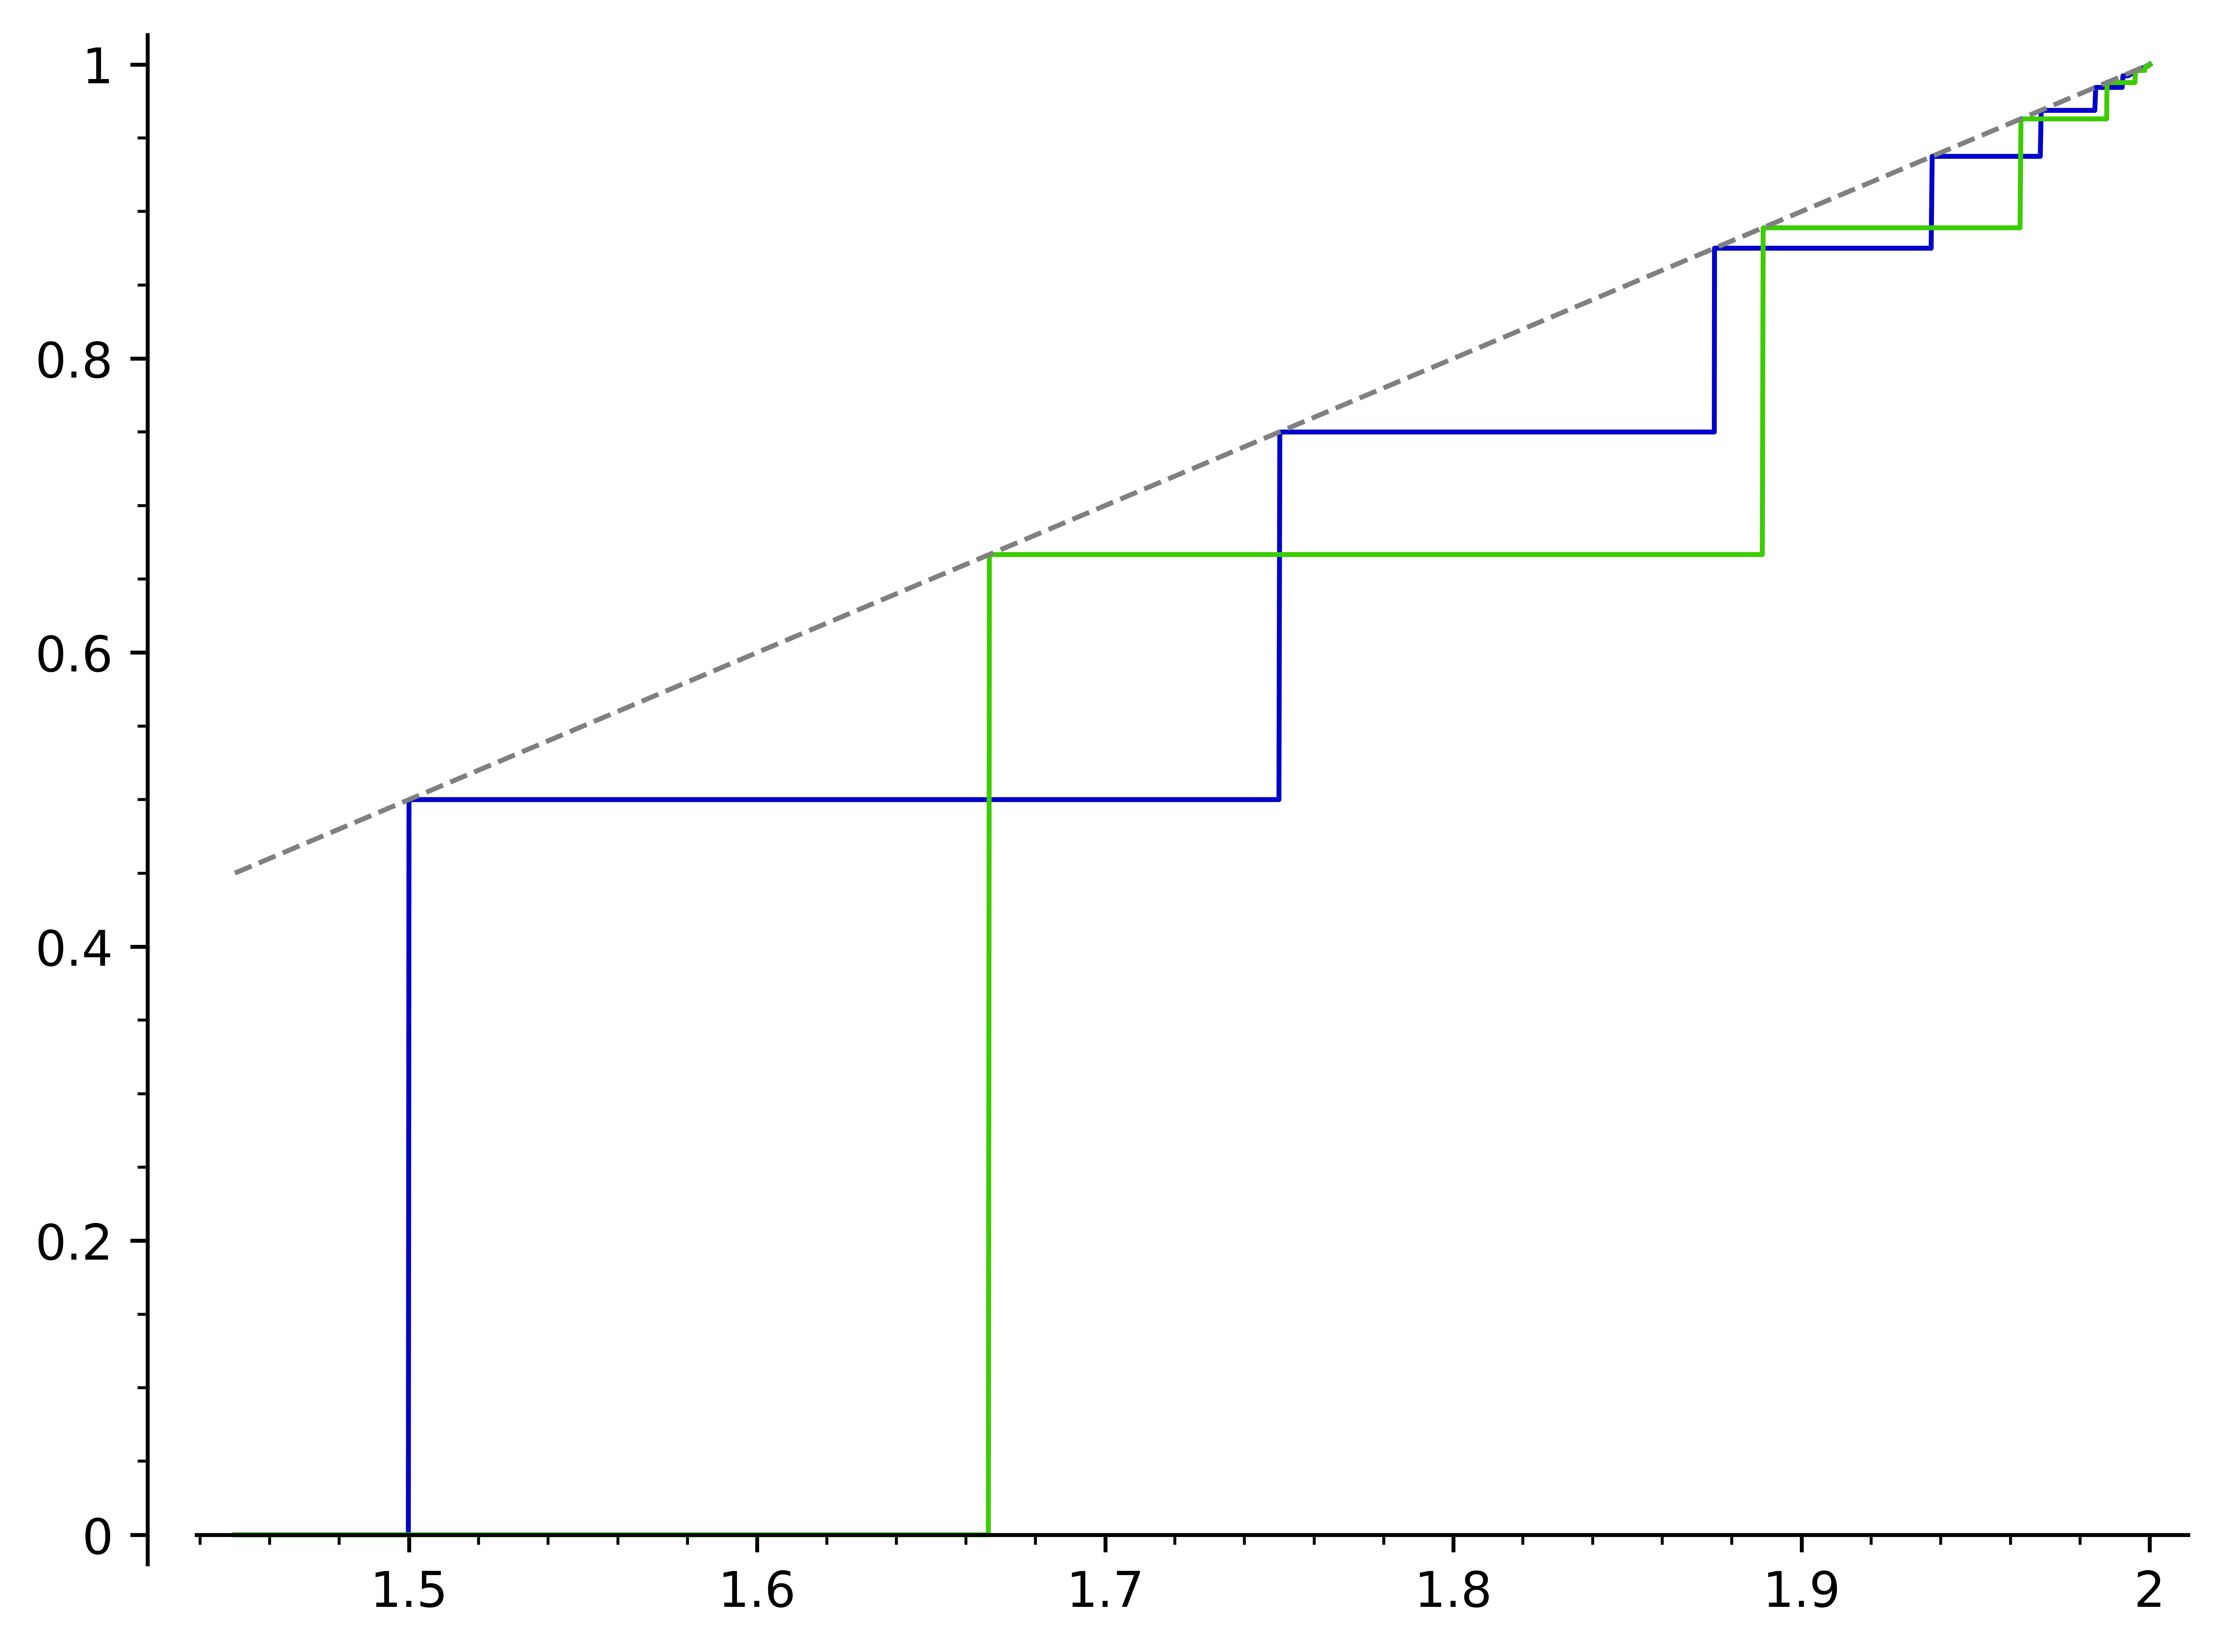
\includegraphics[width=0.5\linewidth]{Pictures/geometric-series-distribution-2-3-half.png}
                \caption{Distribution functions $F_2, F_3$ of geometric series construction}
                \label{fig:distributionsGeometricSeriesCounterexample-2-3}
            \end{figure}
        
            \item 
            In another, more general approach, we start with some discrete distribution $P$ with $\supp P = \set{s_1, s_2, \dots} \subseteq [a, b)$, $1 < a < b$, the $s_i$ in increasing order, and probability mass function $f$ which is monotonic on the support, i.e. $\forall i < j: f(s_i) > f(s_j)$. We construct $\tilde{P}$ with mass function $g$, where each support point is shifted a bit to the right, with its probability adjusted to be only a little smaller, giving the remaining probability mass to the point $\tilde{a} \coloneqq \frac{1+a}{2}$.
            First, set $\tilde{s}_i \coloneqq \frac{s_i+ s_{i+1}}{2}$.
            We adjust the probability of $\tilde{s}_i$ by a factor $c_i < 1$, i.e. $g(\tilde{s}_i) = c_i f(s_i)$, chosen such that $c_i \geq \frac{s_i}{\tilde{s_i}}$ (ensuring $\tilde{P}$ has greater moments than $P$), $c_i \geq 1-\frac{1}{2^i}$ (ensuring the distribution functions alternate), and $c_i \geq \frac{f(s_{i+1})}{f(s_i)}$ (ensuring that $g$ 
            also is monotonic on its support). In summary, we have:            
            \begin{gather*}
                g(\tilde{s}_i) = c_i f(s_i), \quad
                c_i \coloneqq \max\biggset{\frac{s_i}{\tilde{s_i}}, 1-\frac{1}{2^i}, \frac{f(s_{i+1})}{f(s_i)}} < 1, \quad
                g(\tilde{a}) = \sum_{i \geq 1} (1-c_i) f(s_i)
            \end{gather*}
            By the first property of $c_i$, $g(\tilde{s}_i)\tilde{s}_i \geq f(s_i)s_i ~\forall i$, so for the moments we have:
            \begin{multline*}
                m_n(\tilde{P}) - m_n(P)
                = g(\tilde{a})*\tilde{a}^n + \sum_{k \geq 1} g(\tilde{s}_i) \tilde{s}_i^n - f(s_i) s_i^n \\
                \geq g(\tilde{a}) + \sum_{k \geq 1} f(s_i) s_i^n * (\tilde{s}_i^{(n-1)} - 1)
                \geq g(\tilde{a}) > 0
%                \label{eq:momentPushingExample}
            \end{multline*}
            Secondly, the distribution functions alternate: on the one hand, 
            \begin{multline*}
                G(\tilde{s_k}) 
                = g(\tilde{a}) + \sum_{i=1}^k f(s_i)c_i 
                = g(\tilde{a}) - \bigpars{\sum_{i=1}^k (1-c_i) f(s_i)} + F(s_k) \\
                = \bigpars{\sum_{i \geq k+1} (1-c) f(s_i)} + F(s_k) > F(s_k) = F(\tilde{s_k})
            \end{multline*}
            On the other hand, 
            \begin{multline*}
                G(s_k)
                = g(\tilde{a}) + \sum_{i=1}^{k-1} f(s_i)c_i 
                = g(\tilde{a}) + \sum_{i=1}^{k-1} f(s_i) - \sum_{i=1}^{k-1} f(s_i) (1-c_i) \\
                = F(s_k) - f(s_k) + g(\tilde{a}) - \sum_{i=1}^{k-1} f(s_i) (1-c_i) 
                = F(s_k) - f(s_k) + \sum_{i \geq k} f(s_i) (1-c_i)
            \end{multline*}
            Using the second property of $c_i$ and monotonicity of $f$, we get
            $\sum_{i \geq k} f(s_i) (1-c_i) \leq \sum_{i \geq k} f(s_i) \frac{1}{2^i} < \frac{1}{2^{k-1}} f(s_k) \leq f(s_k)$,
            therefore $G(s_k) < F(s_k)$.
            So $P \lesstail \tilde{P}$, and their probability mass, as well as distribution functions are infinitely alternating, such that the sufficient condition of Theorem \ref{thm:acTailOrderSuffConditions} is not satisfied for any $x_0$.
            Furthermore, $\tilde{P}$ again satisfies the conditions we originally made on $P$: by repeating the process, we get a whole sequence of distributions which is ascending wrt. $\lesstail$, and no two consecutive distribution in it satisfy the sufficient condition of \ref{thm:acTailOrderSuffConditions}.
            \label{item:discreteSufficientTailOrderConditionCounterexample}
            
            \item 
            For the absolutely continuous counterexample, we start with two discrete distributions $P_1, P_2$ where $P_2$ is obtained from $P_1$ by the process from \ref{item:discreteSufficientTailOrderConditionCounterexample}: In particular, we require $P_1 \lesstail P_2$, $\supp(P_1) = \set{s_1, s_2, \dots}$, $\supp(P_2) = \set{t_0, t_1, t_2, \dots}$ with $1 < t_0 < s_1 < t_1 < s_2 < t_2 < \dots$ ($t_0$ represents $\tilde{a}$ from above), and their distribution functions $F, G$ should alternate with $F(s_k) > G(s_k), F(t_k) < G(t_k) ~\forall k\geq 1$.
%            their mass functions $f, g$ should satisfy $f(s_i)s_i < g(t_i)t_i ~ \forall i$ (and therefore 
            
            We then shift the probability mass $P_1$ gives to each point $s_k$ to an interval to the left of $s_k$, and the probability mass $P_2$ gives to each point $t_k$ to an interval to the right of $t_k$, which preserves the order of the moments. We do it in such a way that the distribution functions are again alternating, and the new density functions are continuous. We will call the new absolutely continuous distributions $\tilde{P}_1, \tilde{P}_2$, their new density functions $\tilde{f}, \tilde{g}$, and their distribution functions $\tilde{F}, \tilde{G}$.
            
            To formalize this, let $h: \R \to \R, x \mapsto (6x - 6x^2)\1_{[0, 1]}(x)$. $h$ is a simple probability density function ($\lintegral{\R}{h}{\lambda} = 1$), which is continuous since $h(0) = h(1) = 0$.
            Denote by $h_{[a, b]}: x \mapsto \frac{1}{b-a}h\bigpars{\frac{x-a}{b-a}}$ the version of $h$ scaled to the interval $[a, b]$, still integrating to 1.
%            Define $h_{a, b, s}: x \mapsto s*h(\frac{x-b}{b-a})*s$.
%            Another way to view it is that the integral of $h$ continuously interpolates between the values 0 and 1 on the interval $[0, 1]$.
            Also, let $m_{k} = \frac{t_{k-1} + s_k}{2}$.
            Using this notation, we define $\tilde{f}, \tilde{g}$ by:
            \begin{gather}
                \tilde{f} = \sum_{k \geq 1}  f(s_k) h_{[m_k, s_k]}, \quad
                \tilde{g} = \sum_{k \geq 0}  g(t_k) h_{[t_k, m_{k+1}]}
                \label{eq:acSufficientTailOrderConditionCounterexample-densitiesDefinition}
            \end{gather}
            By construction, it's clear that $\lintegral{\R}{\tilde{f}}{\lambda} = \lintegral{\R}{\tilde{g}}{\lambda} = 1$, since $(f(s_k))_{k \geq 1}, g(t_k))_{k \geq 0}$ sum to $1$. The distribution functions are alternating:
            For $k \geq 1$,
            \begin{gather*}
                \tilde{F}(s_k) 
                = \lintegral{[1, s_k]}{\tilde{f}}{\lambda} 
                = \sum_{i=1}^{k} f(s_k) 
                = F(s_k)
                > G(s_k)
                = \sum_{i=1}^{k-1} g(t_k) 
                = \tilde{G}(s_k)
                ,\\                
                \tilde{G}(m_{k+1})                
                = \lintegral{[1, m_{k+1}]}{\tilde{g}}{\lambda} 
                = \sum_{i=1}^{k} g(t_k)
                = G(t_k)
                > F(t_k)
                = \sum_{i=1}^{k} f(s_k) 
                = \tilde{F}(m_{k+1})
            \end{gather*}
            The ordering of the moments is preserved:
            \begin{multline*}
                m_n(\tilde{P_1})
                = \sum_{k \geq 1} \lintegral{[m_k, s_k]}{x^n h_{[m_k, s_k]}(x)}{\lambda(x)}
                < \sum_{k \geq 1} f(s_k)*s_k^n \\
                = m_n(P_1)
                < m_n(P_2) \\
                = \sum_{k \geq 0} g(t_k)*t_k^n
                < \sum_{k \geq 0} \lintegral{[t_k, m_{k+1}]}{x^n h_{[t_k, m_{k+1}]}(x)}{\lambda(x)}
                = m_n(\tilde{P_2})
            \end{multline*}
            If the series in \eqref{eq:acSufficientTailOrderConditionCounterexample-densitiesDefinition} converges uniformly, continuity is preserved.
            For this we need to have $\norm{f(s_k) h_{[m_k, s_k]}}_\infty = \frac{f(s_k)}{s_k - m_k} \toinfty{k} 0$, and similarly for $g$, which is the case if the probability masses $f(s_k)$ approach zero asymptotically faster than the consecutive differences of the $s_k$. For example, we can set $s_k = 2-\frac{1}{k+1}, f(s_k) = \frac{1}{2^k}$, and use $g, (t_k)_k$ constructed from it as in \ref{item:discreteSufficientTailOrderConditionCounterexample}.
            % TODO properly reference “uniform convergence preserves continuity”
        \end{enumerate}
    \end{ex}
    
    
    \chapter{Tweaking the Stochastic Order: Segmenting Loss Distributions}
    
    
    \chapter{Distribution-Valued Game Theory in Security of Critical Infrastructures}
    
%    \nocite{*}
%    \printbibliography
\end{document}